\documentclass[runningheads,a4paper]{llncs}



\usepackage{amsmath}
\usepackage{algpseudocode}
\usepackage{algorithm}
%\usepackage[showframe]{geometry}%<--- only to show the page structure

\usepackage[american]{babel}

\usepackage{graphicx}
\usepackage{lipsum}

%extended enumerate, such as \begin{compactenum}
\usepackage{paralist}

%put figures inside a text
%\usepackage{picins}
%use
%\piccaptioninside
%\piccaption{...}
%\parpic[r]{\includegraphics ...}
%Text...

%Sorts the citations in the brackets
%\usepackage{cite}

%for easy quotations: \enquote{text}
\usepackage{csquotes}

\usepackage[T1]{fontenc}

%enable margin kerning
\usepackage{microtype}

%better font, similar to the default springer font
\usepackage[%
rm={oldstyle=false,proportional=true},%
sf={oldstyle=false,proportional=true},%
tt={oldstyle=false,proportional=true,variable=true},%
qt=false%
]{cfr-lm}
%
%if more space is needed, exchange cfr-lm by mathptmx
%\usepackage{mathptmx}

%for demonstration purposes only
\usepackage[math]{blindtext}

\usepackage[
%pdfauthor={},
%pdfsubject={},
%pdftitle={},
%pdfkeywords={},
bookmarks=false,
breaklinks=true,
colorlinks=true,
linkcolor=black,
citecolor=black,
urlcolor=black,
%pdfstartpage=19,
pdfpagelayout=SinglePage
]{hyperref}
%enables correct jumping to figures when referencing
\usepackage[all]{hypcap}

\usepackage[capitalise,nameinlink]{cleveref}
%Nice formats for \cref
\crefname{section}{Sect.}{Sect.}
\Crefname{section}{Section}{Sections}
\crefname{figure}{Fig.}{Fig.}
\Crefname{figure}{Figure}{Figures}

\usepackage{xspace}
%\newcommand{\eg}{e.\,g.\xspace}
%\newcommand{\ie}{i.\,e.\xspace}
\newcommand{\eg}{e.\,g.,\ }
\newcommand{\ie}{i.\,e.,\ }

%introduce \powerset - hint by http://matheplanet.com/matheplanet/nuke/html/viewtopic.php?topic=136492&post_id=997377
\DeclareFontFamily{U}{MnSymbolC}{}
\DeclareSymbolFont{MnSyC}{U}{MnSymbolC}{m}{n}
\DeclareFontShape{U}{MnSymbolC}{m}{n}{
    <-6>  MnSymbolC5
   <6-7>  MnSymbolC6
   <7-8>  MnSymbolC7
   <8-9>  MnSymbolC8
   <9-10> MnSymbolC9
  <10-12> MnSymbolC10
  <12->   MnSymbolC12%
}{}
\DeclareMathSymbol{\powerset}{\mathord}{MnSyC}{180}

%improve wrapping of URLs - hint by http://tex.stackexchange.com/a/10419/9075
\makeatletter
\g@addto@macro{\UrlBreaks}{\UrlOrds}
\makeatother

% correct bad hyphenation here
\hyphenation{op-tical net-works semi-conduc-tor}

\begin{document}

%Works on MiKTeX only
%hint by http://goemonx.blogspot.de/2012/01/pdflatex-ligaturen-und-copynpaste.html
%also http://tex.stackexchange.com/questions/4397/make-ligatures-in-linux-libertine-copyable-and-searchable
%This allows a copy'n'paste of the text from the paper
\input glyphtounicode.tex
\pdfgentounicode=1

\title{Big Data with High Performance Computing (HPC)}
%If Title is too long, use \titlerunning
%\titlerunning{Short Title}

%Single insitute
\author{Tarek El-Ghazawi \and Krunal Puri \and Armin Mehrabian}
%If there are too many authors, use \authorrunning
%\authorrunning{First Author et al.}
\institute{George Washington University}

%Multiple insitutes
%Currently disabled
%
\iffalse
%Multiple institutes are typeset as follows:
\author{Tarek El-Ghazawi\inst{1} \and Krunal Puri\inst{1} \and Armin Mehrabian \inst{1} }
%If there are too many authors, use \authorrunning
%\authorrunning{First Author et al.}

\institute{
George Washington University\\
\email{...}\and
Insitute 2\\
\email{...}
}
\fi
			
\maketitle

\begin{abstract}
Abstract goes here
\end{abstract}

\keywords{...}

%%%%%%%%%%%%%%%%%%%%%%%%%%%%%%%%%%%%%%%%%%%%%%%%%%%%%%%%%%%%%%%%%%%%%%%%%%%%%%%
\section{Introduction}\label{sec:intro}
%%%%%%%%%%%%%%%%%%%%%%%%%%%%%%%%%%%%%%%%%%%%%%%%%%%%%%%%%%%%%%%%%%%%%%%%%%%%%%%
%\blindtext
For a long time the terms Big Data and High Performance Computing (HPC) have been used interchangeably implying that they convey the same meaning. Many experts take this even further and recognize HPC as the entity that gave birth to Big Data. However, the two seem to have chosen separate paths fueled by two different driving forces namely, scientific community and industry. HPC has its roots in computation-intensive scientific modeling performing iterative algorithms. In contrast, Big Data was born as a result of a demand for gaining insight from large unstructured data stored by industries and nowadays by us human beings digital life. But, as data generation rate out-paces its processing workforce, Big Data solutions face an inevitable require to adopt more advance processing approaches having higher efficiency and performance.  As a result the boundary between HPC and Big Data is fading everyday. Authors believe that the gap between Big Data and HPC may form a spectrum of choices rather than two independent worlds. In this chapter we will first bring a brief introduction on Big Data and HPC then we will take and look at big data and HPC from a high level abstraction view. The majority of this chapter is dedicated to state of the art efforts to take advantage of the best of two worlds. Finally, we will address future challenges and future directions.\\

\begin{figure}
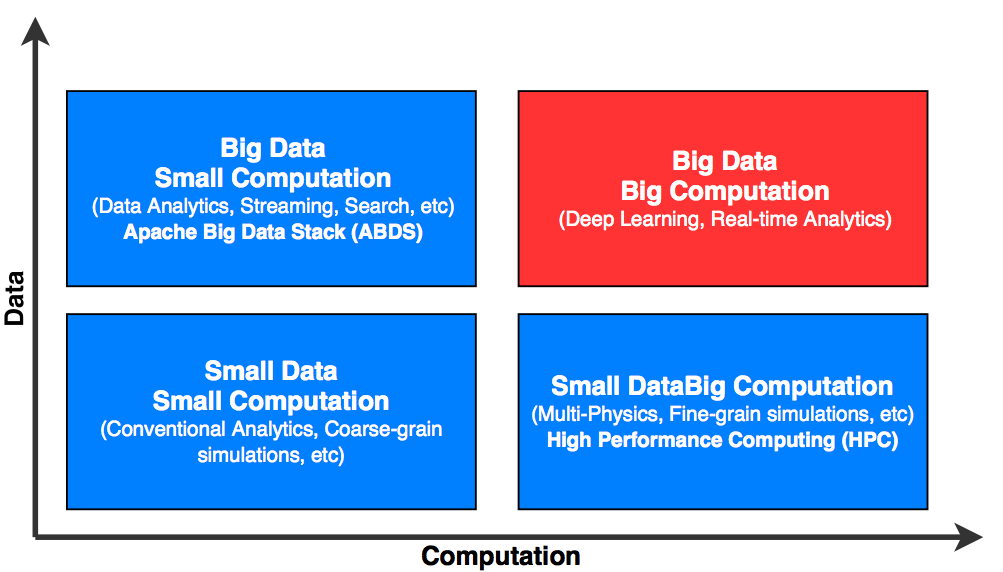
\includegraphics[width=\textwidth]{./images/bigdata_matrix.png}
\centering
\caption{Matrix of data and computation applications.}
\label{fig:bigdata_hpc_matrix}
\end{figure}
In order to address the above issues we first may need to identify the workloads and computational requirements of workflows for each application. It is also important to not focus only on current trends, and take into account the future data and computation demands. Figure \ref{fig:bigdata_hpc_matrix} shows the matrix of data size versus computation size for some applications. It also shows that the current big data technologies is data-intensive but focused less on computational performance. On the other hand the High Performance Computing (HPC), which mostly applied to solving scientific problems and fine-tuned for particular problems, has been mostly concentrated on computation-savvy, data limited application such and iterative simulations commonly used to solve scientific problems.\\


\subsection{Big Data Ecosystem}
Big data is commonly distinguished by its 5V properties namely, Volume, Variety, Velocity, Value, and Veracity. However, Vs are not the only factors impacting the architecture of a big data ecosystem. In \cite{demchenko2014defining} Demchenko \textit{et al.} propose a definition of big data characteristics and requirements in five categories. These categories are, 5V properties, new data models, new data analytics, new infrastructures, and new data sources and targets. Therefore, a big data ecosystem should be able to address the problems introduced by each of these properties.\\

It should be noted that there has not been a well accepted definition of big data either by industry or academia. This ambiguity makes it even harder to characterize big data and define requirements of a big data ecosystem. In addition, big data ecosystem is not merely made out of a single or couple of components such as a file system or a database. A big data ecosystem should account for lots of components from storage and processing to orchestration and high level applications. Figure \ref{fig:bigdata_ecosystem} depicts a generic architecture of a big data ecosystem.

\begin{figure}
	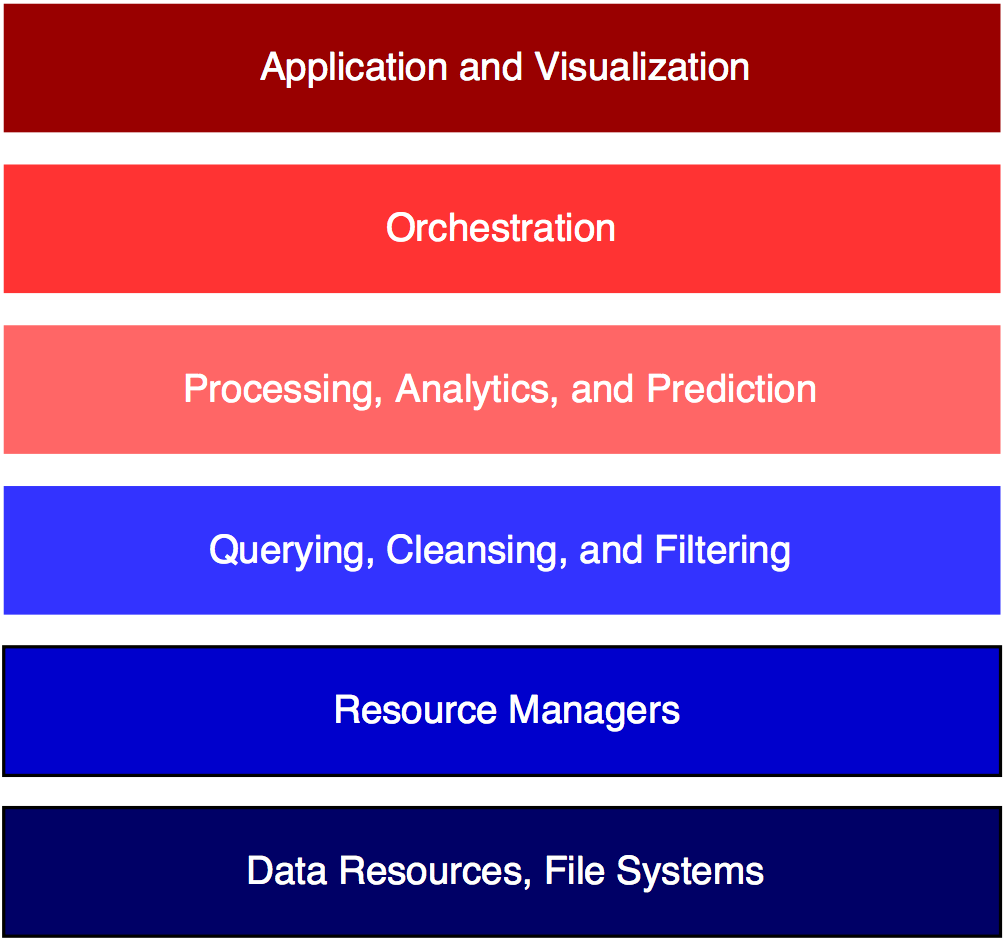
\includegraphics[scale=0.23]{./images/bigdata_ecosystem.png}
	\centering
	\caption{A general big data ecosystem architecture.}
	\label{fig:bigdata_ecosystem}
\end{figure}



\subsubsection*{ABDS Architectures}
The Apache Big Data Stack is formed around the Hadoop Distributed File System (HDFS), which originated at Yahoo but is an open source implementation of Google's file system \cite{shvachko2010hadoop} \cite{ghemawat2003google}. As we know now, the idea behind ABDS was to bring the computation to data, which is usually stored at cheap commodity heterogeneous hardware. Apache Hadoop 1.0 adopted Google's MapReduce programming model for data processing. MapReduce imposes its own limitations since all processes are forced to be implemented in the form of a mapper and a reducer. MapReduce's inherent limitations along with tight coupling of Hadoop and MapReduce proved to be inflexible when used in applications such as iterative computations, which is an essential piece of most of higher level analytics such as Machine Learning algorithms. Figure \ref{fig:ABDS_ecosystem} depicts the ABDS ecosystem.\\

\begin{figure}
	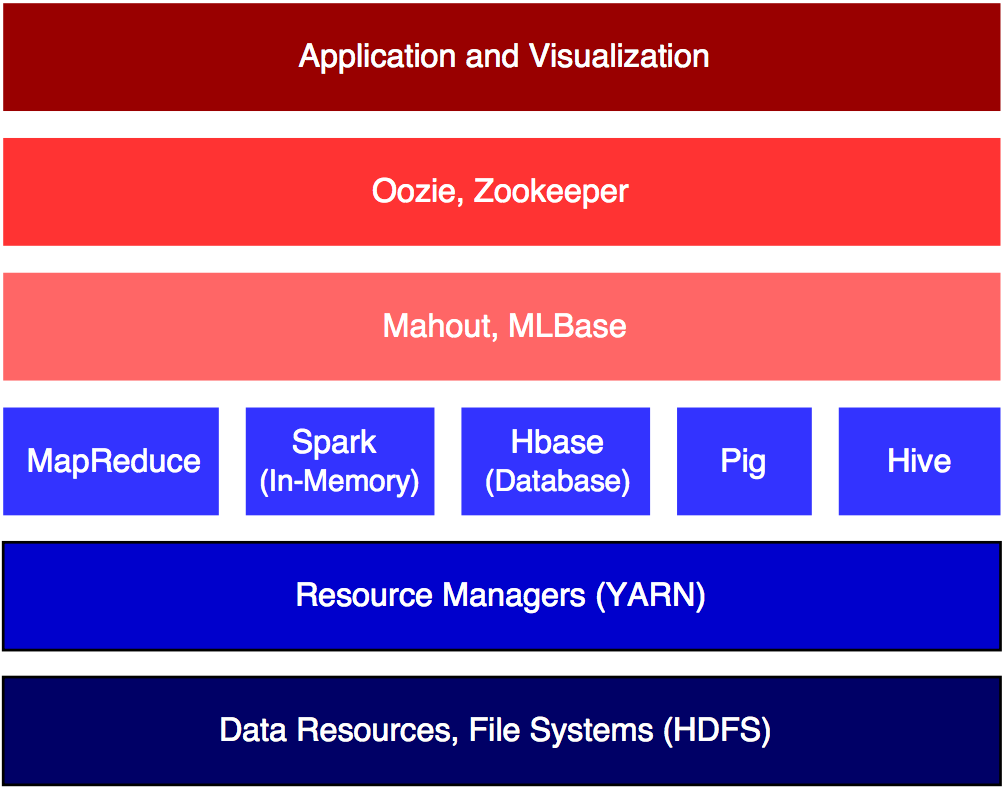
\includegraphics[scale=0.23]{./images/abds_ecosystem.png}
	\centering
	\caption{Apache Big Data Stack (ABDS) ecosystem.}
	\label{fig:ABDS_ecosystem}
\end{figure}

As a result of such shortcomings of Hadoop 1.0, Apache YARN was introduced with Hadoop 2.0 as a much more lenient resource manager, enabling many applications and frameworks with higher level abstractions \cite{vavilapalli2013apache}. YARN's key feature was introduction multi-level scheduling, which would allow higher level applications to schedule their own processes. As a results we saw the emerge of many high level applications such as, HBase, a column based distributed database, Spark, Giraph, which are iterative and graph processing applications respectively\cite{borthakur2011apache}\cite{zaharia2012resilient}.

\subsection{HPC Ecosystem}

A typical HPC architecture consists of processing units such a multi-core structures, possibly accelerated by GPUs, FPGAs, or even CPUs such as intel Xeon Phi. These processing units are supported by local storage units with Lustre \cite{braam2004lustre} or General Parallel File System (GPFS) \cite{FrankSchmuck} file system or a remote storage connected through a fast network such as Infiniband. Figure \ref{fig:HPC_ecosystem} shows an example of a typical HPC ecosystem.\\

\begin{figure}
	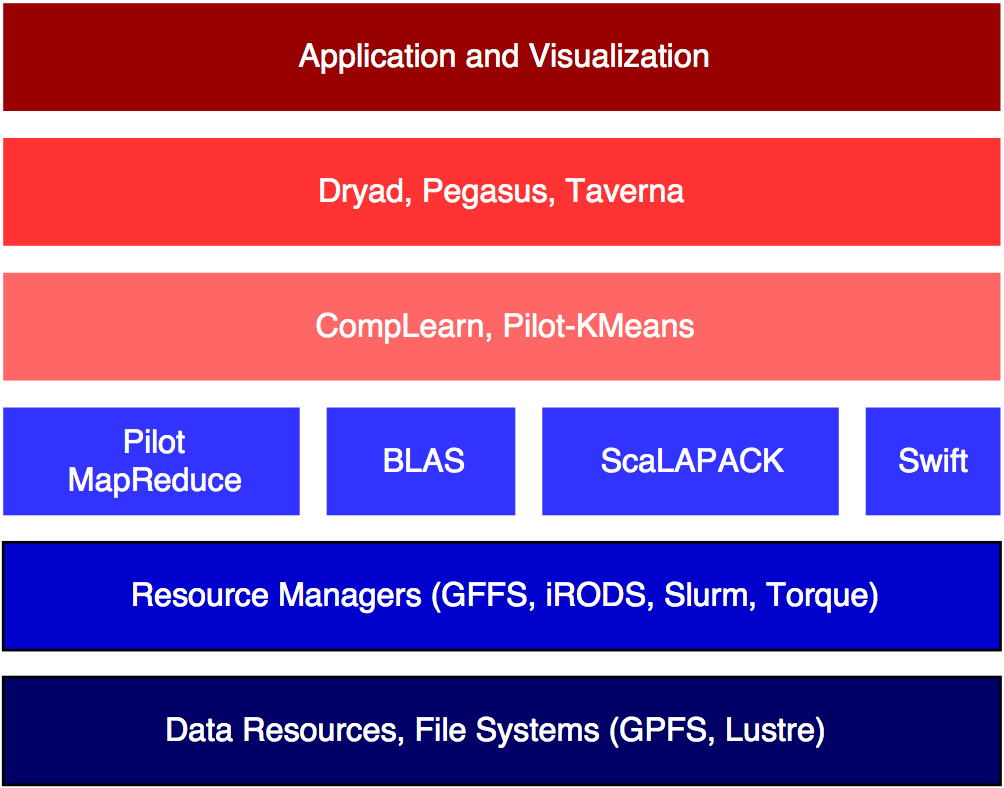
\includegraphics[scale=0.23]{./images/hpc_ecosystem.png}
	\centering
	\caption{An example of HPC ecosystem.}
	\label{fig:HPC_ecosystem}
\end{figure}

Lustre and GPFS are parallel file systems designed mainly for clusters. Lustre, which combines the words Linux and Cluster is generally accepted as the file system with scalability for large scale cluster computing. Due to its high performance it has been continuously used by top supercomputers. On the other hand GPFS introduced by IBM and adopted by many of the biggest companies all around the word. GPFS have it roots in academic grounds and its scalability is a matter of question. Storage resources in HPC are managed by storage management unit such as integrated Rule-Oriented Data-management System (iRODS), Storage Resource Manager interface (SRM) \cite{shaun2007storage} \cite{rajasekar2010irods},  Global Federated File System (GFFS) \cite{grimshaw2013gffs}.\\

While storage resources are usually shared in applications, computational resources are local. Such local compute resources are managed by their own management units such as Slurm \cite{yoo2003slurm}, Torque \cite{staples2006torque}, and Sun Grid Engine (SGE) \cite{gentzsch2001sun}.

In HPC applications, data need to fly around across network using a low latency communication. These fast interconnect networks along with features such as non-blocking and one-sided communications allow for more data-intensive HPC within HPC environment. As a matter of fact, data-intensive applications are not totally unfamiliar to HPC community. There has been many approaches to implement MapReduce compatible with HPC environment such as MapReduce-MPI \cite{plimpton2011mapreduce}, Pilot-MapReduce \cite{mantha2012pilot}, and Twister for machine learning applications \cite{ekanayake2010twister}.In a parallel effort, there has been many implementations of data intensive loosely coupled tasks at run-time level \cite{luckow2012p}\cite{raicu2008many}\cite{deelman2009workflows}.
 
\subsection{Big Data Applications}
In the beginning of the twenty first century data mining and data processing became the driving force behind many fields such as business, Information Technology (IT), etc. Over the recent past Big Data has risen to address the many large-scale data driven problems, which formerly viewed as unsolvable. In this part we will briefly discuss these applications in two major environments namely, commercial and scientific environments.\\

\textit{Big Data Commercial Applications:} Since 90s until the recent present, most of the data stored by companies were in the form of relational databases. However, nowadays with the enormous data generated in various forms such as activity logs, pictures, audio, clicks, and lot of other types, old database paradigms proved to be inefficient. As a results big data analytics with non-relational databases, distributed storages, secure and fault tolerant architectures have gained momentum in data analytics from data storing, data cleansing, to complicated statistical analysis for predictive analytics and visualization. In parallel, fields such as Machine Learning and Deep Learning where data is the driving thrust, benefited the most from Big Data. This trend introduced and revived many applications within Artificial Intelligent (AI) realm. The synergy between the AI and dominance of web based applications working with unstructured data has already discovered new universe of applications such as videos surveillance for law enforcements and intelligence agencies, recommendation engines for personalized shopping, etc. \\


\textit{Big Data Scientific Applications:} Scientific communities acquaintance with big data predates industry. Particle physics, Astrophysics, Genetics, Meteorology, and lot of other fields have been dealing with massive amounts of data, most of the times beyond their processing power. Recently, the National Science Foundation (NSF) announced the Big Data research initiative and called the researches to extract knowledge and insight from data.
\subsection{Integration of big data and HPC ecosystems}
Traditional data analytics in the past have been able to extract general high level information from data. But, as the data started to generated with the 5V properties, those old method proved to be less and less effective. Consequently, many data consumers have pointed their short-term and long-term agendas towards implementation and adoption of new methods of data analysis.\\

Despite Big Data and HPC's different contexts, HPC has a relatively long history addressing many of these challenges. HPC is conventionally built around the expensive supercomputers including a large number of servers. On the other hand Big Data has its roots in commodity hardware focusing on priorities such a fault tolerance, scheduling, and heterogeneous computing. HPC components are usually tightly coupled as opposed to its loosely coupled big data counterpart. It is evident that in order to take advantage of the best of the two worlds, we need some breakthroughs in HPC to provide more heterogeneous computing power and Big Data to embrace more efficient components from HPC.\\

In addition, HPC and big data communities have favored different programming models. Due to shortcomings of MPI alone, which is incapable of scaling at Exascale, current trend in HPC is to take advantage of MPI+X as runtime communication libraries. These libraries require to support many MPI+X combinations such as MPI+OpenMP, MPI+UPC, MPI+SHMEM, etc. It should be noted that at Exascale such libraries should be able to provide inter/intra node communications for billion processors.  


\section{State of the art projects}
In this section we will review some of the state of the art researches and projects within HPC-Big Data domains. We categorized these project under four class of research topics, namely,
\begin{enumerate}
	\item Integration of HPC and ABDS stack
	\item Machine Learning (ML) using HPC
	\item High Performance Graph processing
	\item Parallel databases
	\item HPC implementation of MapReduce 
	
\end{enumerate}
\subsection{Integration of HPC and big data stack}
Earlier in this chapter we discussed how HPC can offer many solutions to Big Data's current challenges. In this section we review a state of the art effort to combine HPC and Big Data ecosystem under {High Performance big data System (HPBDS) project. 

\subsubsection{High Performance Big Data System (HPBDS) project \cite{qiu2014towards}}: The HPBDS project aims for combining some of the components of the HPC such as scientific libraries, fast communication and resource management features with commercial Big Data ecosystem namely, ABDS.\\

The proposed design of HPBDS is built around the commercial Apache Hadoop project and therefore named High Performance Computing Big Data Stack (HPC-ABDS). The HPC-ABDS comprise two sub-project,
\begin{figure}[h]
	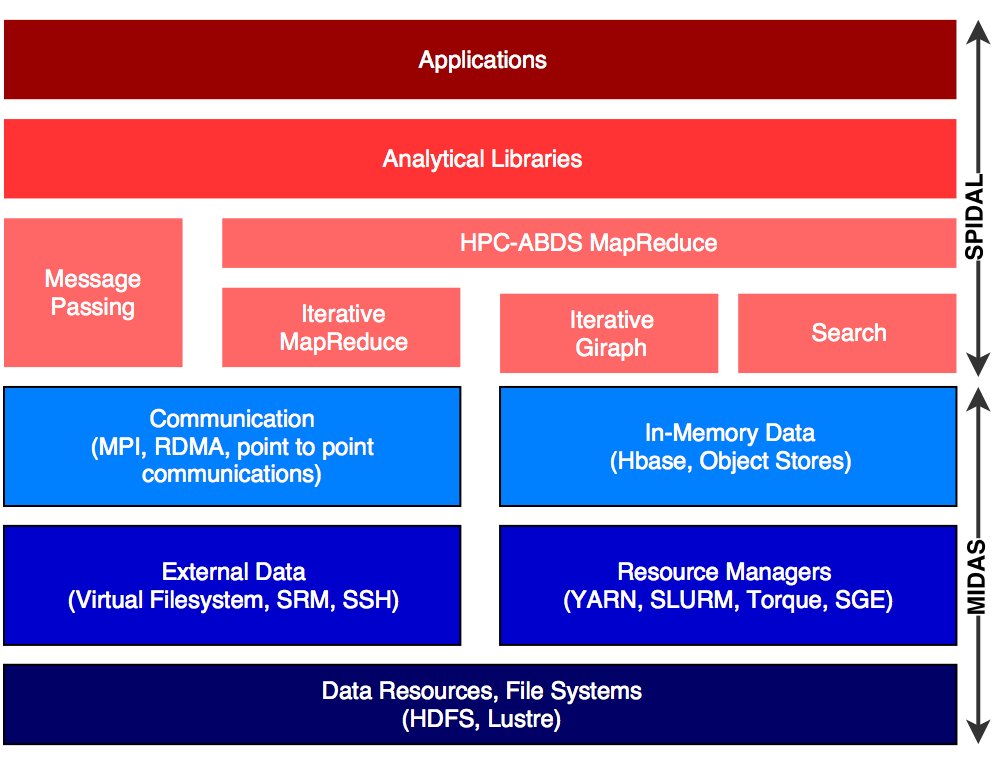
\includegraphics[scale=0.25]{./images/hpc_abds.png}
	\centering
	\caption{MIDAS and SPIDAL within HPC-ABDS stack\cite{qiu2014towards}}
	\label{fig:MIDAS_SPIDAL}
\end{figure}
\begin{enumerate}
	\item Scalable Parallel Interoperable Data Analytics Library (SPIDAL)
	\item Middleware for Data Intensive Analytics and Science (MIDAS)  
\end{enumerate}

Figure \ref{fig:MIDAS_SPIDAL} depicts the structure of the MIDAS-SPIDAL with respect to the overall HPC-ABDS stack. MIDAS is proposed to provide a lower level infrastructure based on which higher level components such as libraries operates. MIDAS aims to couple performance of HPC with functionality of heterogeneity of Apache Hadoop tools. On the other hand SPIDAL goal is to take advantage of useful tool within HPC such as MPI, PETSc, and SCALAPACK and modify them for data intensive applications.\\

The HPC-ABDS project is inspired by the NIST big data initiative in Fall 2013, when NIST provided a collection of use cases. These use cases were analyzed against the identifiers proposed as big data Ogres \cite{fox2014towards}. Based on the results from analyzing 71 use cases provided by NIST against data Ogres, five programing models was established. Table \ref{table:NIST_5_Programming_model} summarizes these programming models. 

%%%%%%%%%%%%%%%%%%%% EXACTT %%%%%%%%%%%%%%%%%%%%%%%%%%%%%%%%%%%%%%%%%%%%%
\begin{table}
	\centering
	\caption{Five programming models identified for big data HPC problems based on NIST big data use cases.}
	\begin{tabular}{ |p{4cm}|p{7cm}|  }
		\hline
		\textbf{Programming Model} & \textbf{Description} \\
		\hline
		Pleasingly Parallel & Applications such as local machine learning where processing is applied over many items in a local machine. Either Hadoop or other HPC tools could be used. \\
		\hline
		Classic MapReduce & Including MRStat, some search applications, collaborative filtering and motif finding. Traditional Hadoop and MapReduce could be used.\\
		\hline
		Iterative Map Collective & Iterative applications of MapReduce using collective communication. Hadoop 2.0 along with tools such as Spark could be used.\\
		\hline
		Iterative Map Communication & Iterative MapReduce such as Giraph with pointto-point
		communication, includes most graph algorithms
		such as maximum clique, connected
		component, finding diameter, community detection).
		 \\
		\hline
		Shared Large Memory & Thread-based (event driven) graph algorithms
		such as shortest path and Betweenness centrality.
		Large memory applications.\\
		\hline
		
	\end{tabular}
	\label{table:NIST_5_Programming_model}
\end{table}

\subsection*{Scalable Parallel Interoperable Data-Analytics Library (SPIDAL) }
SPIDAL project is formed around characteristics identified by analyzing NIST uses cases and programming models in Table \ref{table:NIST_5_Programming_model} to build higher level abstractions based on the middleware analytic tools proposed by MIDAS. The followings comprise  core library category of SPIDAL.
\begin{itemize}
	\item \textbf{Graph and Networks:} With graphs taking over many applications that traditionally did not belong to them, graph processing has become a more and more important. SPIDAL approach for graph processing involve creation of new tools and techniques based on both MapReduce and Giraph \cite{avery2011giraph} model. Graph processing solutions are based on structures withing the graph or network. For a wide range of structures Giraph based solutions seem to better perform mostly when a distributed memory parallel approach is taken. On the other hand a range of graphs respond better to MapReduce solutions when problem can be disintegrated into reduction operations.\\
	\item \textbf{Spacial Queries and Special Analytics:} Spacial Data Management Systems (SDBMS) are incapable of performing tasks that require lots of computations optimally. Thus, the proposed design shards the space into partitions and breaks the most time-consuming partitions into multiple chunks feeding them into parallel MapReduce. Hadoop-GIS \cite{aji2013hadoop} embedded into Apache Hive enables querying on MapReduce.\\
	
	\item \textbf{Image Processing:} Computer vision over the past few years has been empowered by introduction of new tools and techniques such as GPUs and Learning algorithms. In addition, image processing tasks generally tend to be highly parallelizeable. SPIDAL will provide a comprehensive image processing library both at high system level and primitive pre-processing functions and kernels such as Convolution.\\
	 
	\item \textbf{Machine learning:} There are many Machine Learning libraries designed for Apache Hadoop framework. Within Hadoop ecosystem, Apache Mahout supports many of both supervised and unsupervised Machine Learning algorithms. SPIDAL will include a set of key Machine Learning algorithms such as Support Vector Machines (SVM), Random Forests, etc. SPIDAL will try to have Machine Libraries parallelized. Besides, SPIDAL will give those iterative algorithms that require disk I/O in current Big Data environment, a bigger boost in performance.  
\end{itemize}

\subsection*{Middleware for Data Intensive Analytics and Science (MIDAS)}

MIDAS is proposed to facilitate a lower abstraction level, which includes run time and resource management for SPIDAL. We now know from analysis of big data ogres and NIST use cases that big data application vary widely in requirements and characteristics. Therefore, different programming models and parallel approaches should be considered dealing with each type of problems. With this in mind, MIDAS has targeted two major objectives. First, a high abstraction level environment that supports querying and analysis via HPC and big data tools such as SLURM and YARN as schedulers. Secondly, to provide a middleware that support the four of the identified programming models in table \ref{table:NIST_5_Programming_model} namely, Pleasingly Parallel, Classic MapReduce, Iterative Map with Collectives, and Iterative Map Communication. Hence, difference abstraction layers have been recommended. For instance, in applications that better fit the iterative MapReduce, most operations are collective and MPI would perform better compared to MapReduce techniques. In contrast, graph processing application require more point to point communications.\\

In conclusion, HPC-ABDS as claimed by the authors is the first attempt to create a HPC empowered big data stack. The HPC-ABDS tries to find and characterize application patterns through a set of features named as Ogres. A set of libraries (SPIDAL) are created based on characteristics identified by the Ogres run across various computing platforms. SPIDAL runs on MIDAS, which is a middleware with resource management and data abstraction capabilities. 

\subsection{Machine Learning and HPC}
Traditionally the words Machine Learning and HPC would imply two separate worlds with distinct border. But, over the recent past, areas of AI such as machine learning and training neural networks of deep learning have found their ways through HPC world.\\

Iterative AI tools such as machine learning and deep learning initially introduced to HPC through GPU accelerators and FPGAs. These tools were adopted to perform a wide range of AI tasks from image classification, audio recognition, to data analytics. Machine learning is not a novel concept and has been around for a relatively long time. But, along with more computational power introduced by accelerators, two major factors played an undeniable role in re-emergence of machine learning and deep learning. First, data generation at blasting rates fuels up machine learning training algorithms. In a series of reports by Domo, \cite{domo} the amount of data created at the some of the biggest Internet giants, is presented. Table \ref{table:Domo} shows some of these numbers in only one minute time of Internet. Secondly, introduction of new training algorithms, which also gave birth to the term Deep Learning \cite{hinton2006fast}.
\begin{table}
	\centering
	\caption{One minute of Internet usage \cite{domo}.}
	\begin{tabular}{ |p{3cm}|p{9cm}|  }
		\hline
		Company & Count \\
		\hline
		Facebook & Users like \textbf{4,166,667} posts.\\
		\hline
		Twitter & Users send \textbf{347,222} tweets.\\
		\hline
		Youtube & Users upload \textbf{300} hours of video.\\
		\hline
		Instagram & Users like \textbf{1,736,111} photos. \\
		\hline
		Pinterest & Users pin \textbf{9,722} images.\\
		\hline
		Apple & Users download  \textbf{51,000} apps.\\
		\hline
		Netflix & Subscribers stream  \textbf{77.160} hours of video.\\
		\hline
		Reddit & Users cast  \textbf{18,327} votes.\\
		\hline
		Amazon & Receives  \textbf{4,310} unique visitors.\\
		\hline
		Vine & Users play  \textbf{1,041,666} videos.\\
		\hline
		Tinder & Users swipe  \textbf{590,276} times.\\
		\hline
		Snapchat & Users share  \textbf{284,722} snaps.\\
		\hline
		Buzzfeed & Users view  \textbf{34,150} videos.\\
		\hline
		Skype & Users make  \textbf{110,040} calls.\\
		\hline
		Uber & Passengers take  \textbf{694} rides.\\
		\hline
		
	\end{tabular}
	\label{table:Domo}
\end{table}

Deep Learning, which itself is a sub-category of Machine Learning, has gained momentum in solving many of the most complicated AI problems. In many fields such as computer vision and voice recognition Deep Learning outperforms best conventional models and techniques both in accuracy and speed. The major distinguishing difference between most of Machine Learning techniques and that of Deep Learning is in feature selection stage. In conventional Machine Learning, labeled/unlabeled data is fed into a set of hand crafted feature detectors. A classifier takes the features as inputs to perform some statistical analysis and decide on the class of each input. Since the engineering of a good set of such hand crafted features is extremely costly and require a lot of expertise and domain knowledge, Deep Learning is introduced as a solution to find and tune such features automatically using machine and data for a particular task.\\

There is a general consensus that, increasing the size of either or both if training data and/or model size will increase the accuracy of prediction in Deep Learning. Therefore, as the size of training data or the model increases, we require to parallelize the process on many machines and processing cores to enable the scaling. Consequently, two parallelization schemes is offered namely, data parallelization and model parallelization.\\

In data parallelization scheme, the training set is cut into smaller data fragments. Each of these fragments is assigned to a different processing node. Each node replicates the global model so that each model will have a fragment of data with a copy of full model. During the training process the model is updated. Since different copies of the model are updated separately using different fragmentations of data, we need to synchronize all copies of the model into a global model that is representative of all the data. The issue with such synchronizations is the large communication overhead. Models are usually relatively huge (currently up to Gigabytes) that we cannot easily synchronize them frequently. In addition, it is also so hard to fit large models in GPUs' memory.\\

\begin{figure}[h]
	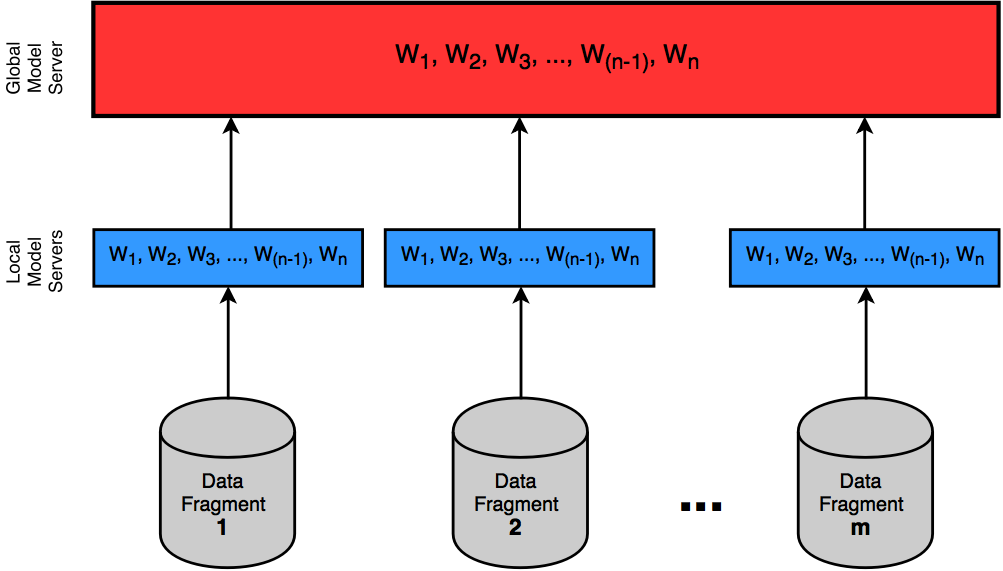
\includegraphics[scale=0.33]{./images/data_parallel.png}
	\centering
	\caption{Data parallelism performing Gradient Descent (GD). Model replicas at each node calculate gradients $\Delta w $ on a piece of data. Gradients are later transmitted to global model server to calculate updated weights.}
	\label{fig:data_parallelism}
\end{figure}
In model parallelization scheme, models are split into smaller pieces, which allows for scaling of the model. A drawback of model parallelization is that one has to synchronize all copies of the model even more frequently than data parallelization. Synchronization should take place for each model at every layer, which for nowadays deep networks can be tens of layers. Thus, interconnects play a very important role when it comes to model parallelization. For instance, a typical neural network architecture with 1 billion nodes may require tens of seconds when using a typical Ethernet networking for synchronization. In contrast, HPC known interconnects such a Infiniband and PCI Express would allow for more efficient networking with higher performance.\\
\begin{figure}[h]
	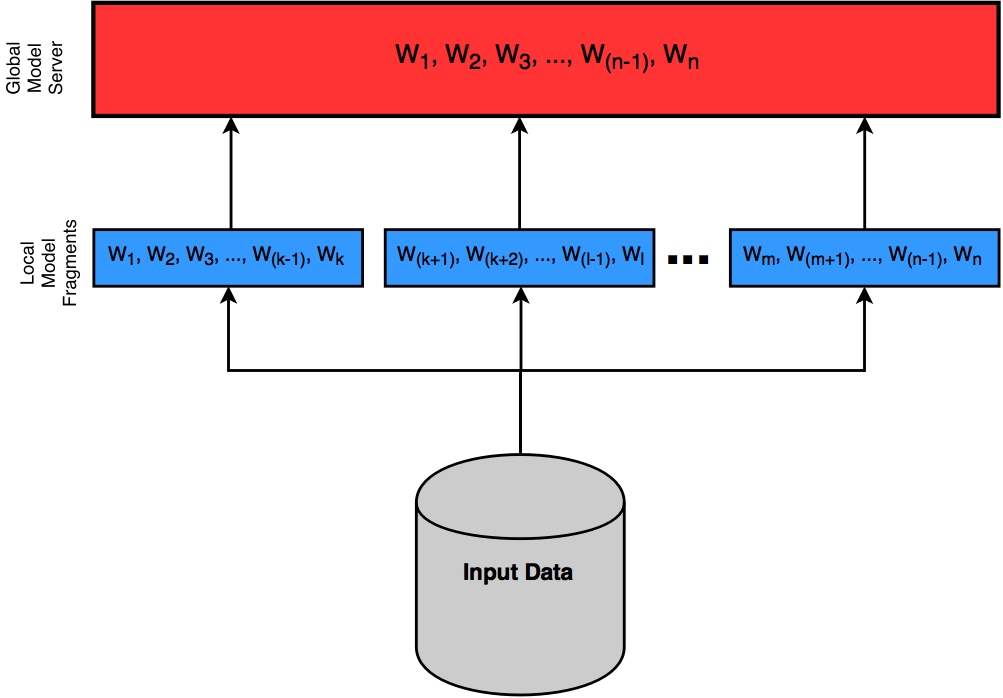
\includegraphics[scale=0.33]{./images/model_parallel.png}
	\centering
	\caption{An example of model parallelism. Each node store a fragment of the overall model and a whole copy of data.}
	\label{fig:model_parallelism}
\end{figure}

There are many crucial issues to be addressed when thinking about integration of Machine Learning and HPC. Questions such as, aside from accelerating Machine Learning with GPUs and FPGAs, is traditional HPC ready to be the drive force behind data savvy Machine Learning applications? Are current top 500 supercomputers capable of powering new AI era of machine learning and Deep Learning? From software point of view, does conventional HPC require extensive modification to deal with mostly correlated data variables in Machine Learning application?
In the remaining of this section we will briefly introduce some of the ongoing researches and projects concentrated empowering Machine Learning with HPC medium.

\subsection*{Project Adam: Building an Efficient and Scalable Deep Learning Training System \cite{chilimbi2014project}}
In 2012 Google announced that they have trained an unsupervised image recognition neural network with 1 billion connections using 10 million training images, which can recognize pictures of cats from Youtube videos. Their training system consisted of a cluster of 1,000 computers with an aggregate of 16,000 cores \cite{le2013building}.\\

Project Adam by Microsoft could be thought as the successor of Google's project. Adam is built using with 30 times less number of machines compared to previous best image classifier. It also is able to train a image classifier using 14 million images of Imagenet \cite{deng2009imagenet} into 22,000 image categories with almost 2 times better accuracy compared to the last best system. Adam is claimed to be 50 times faster than the state of the art systems.\\

\subsection*{High level architecture}
Adam is similar in architecture to the Multi-Spert system introduced by Farber at Berkeley \cite{farber1997parallel}. A set of machine have the role of providing the inputs of the neural network with the input data, while another set train the model. Adam takes advantage of both model and data parallelism. Models machines each hold a chunk of model in a way that the communication overhead between machines is minimized. In order for each piece of the model to be trained only by a small chunk of data, many replicas of the same piece of model in parallel are trained on different data chunks.\\
\begin{figure}[h]
	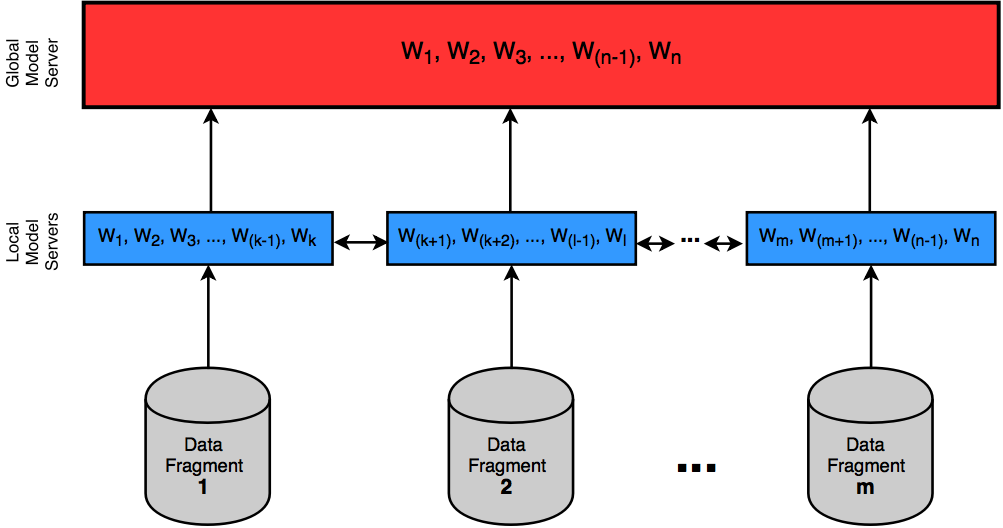
\includegraphics[scale=0.33]{./images/adam_architecture.png}
	\centering
	\caption{Model and data partitioning in Adam architecture\cite{chilimbi2014project}.}
	\label{fig:adam_parallelism}
\end{figure}

A global Parameter Server stores the global values for the updated weights of all model pieces and replicas. The communication between the models and the Partition Server is asynchronous. Although the asynchrony between models and Parameter Servers may seem to introduce inconsistencies, but due to the resilient nature of the neural networks, they usually get trained successfully. As a matter of fact Microsoft researchers found that when they switched from asynchronous to synchronous communication between the models and the Parameter Server, the accuracy of the model dropped. The drop in the accuracy is justified as most of cost functions is datasets such as Imagenet and MNist are not convex functions. As a result, during the training process, the trainer may gets stuck at local optima rather than the global optima. The asynchronous updating of the weights cause the trainer in local optima get some momentum to escape local optima towards a global optima.\\

In traditional neural networks, propagating from one layer to the next layer is equivalent to a mathematical matrix multiplication between the outputs of previous layer and the weights. In some cases there may be other mathematical operations used instead of matrix multiplication. Convolution is one of these operations. Convolutional neural networks are a special type of neural networks that have one or more convolution layers. Such networks are primary choice for image classification and vision since convolutional layers are capable of detecting features. It should be noted that Adam is not merely an image classification system and is capable of training any deep neural network with back-propagation. In Figure \ref{fig:adam_parallelism} each local model server possess some of the convolution and some of the fully connected layers. This type partitioning allows for the communication of the convolution layers across machines to be minimized.\\

Training process on each single machine is multi-threaded. Threads hold activation functions and weights to use during feed-forward and back-propagation through None Uniform Memory Access (NUMA) fashion to reduce the cross-memory bus traffic.\\

Earlier we mentioned that neural networks are resilient so that we could use asynchronous communication between machines and global Parameter Server for updating weights. Same argument could be applied here for weight updates by threads on a single machine. On each machine a shared model holds the weights from all of threads weight updates. In order to avoid the lock times, threads update weights on the shared model without locking. Resilience of the neural networks along with commutativity and associativity properties of weight updates make the model work despite possible overwriting and race conditions of weight updates. This is one of the most important optimizations that allow scaling of deep neural network training process.\\

During the training process weights need to be transmitted back and forth among layers. In order to minimize redundant copies, a pointer is passed along rather than rather than the values. In addition, in the model parallelism architectures, there are some communication between layers across multiple machines. These non-local communications are performed through a library built by project Adam team. The library is custom fit to the communication design of Adam, which supports pointer addressing to blocks of neurons that their output needs communication.\\

The partitioning of the models is Adam is done in a way that the working sets fit inside a L3 cache. Besides, an assembly kernel is implemented and tuned to exploit the locality during feed-forward and back propagation. The kernel allows for optimal matrix multiplication whether row major or column major blocks of weights are to be multiplied.\\

The Global Parameter Server holds the updated weights of the overall model from all machines. Due to high volume of weight updates, the Global Parameter Server of Adam require a more complex design rather than a conventional key value store.\\

Model parameters on the parameter server is partitioned into weight shards of size 1MB. The model partition in the Parameter Server helps with the spatial locality of the updates. In addition, to lower the communication between L3 caches and the parameter server, weight updates are not sent over to the parameter server once they are ready. Instead, weights are batched into blocks and then transferred over to parameter server. To assure the fault tolerance of the processes on the parameter server, there are three copies of weight shards available. One of the shards is assigned as the primary and the other two as the secondary to be used in the primary is cannot be used.\\

Adam is formed of a cluster of 120 machines in three racks connected using IBM G8264 switches. Machine is Adam cluster are servers of HP Proliant servers consisting of dual Intel Xeon E5-2450L processors with 16 cores and 98GB main memory along with two 10Gb NICs and one 1Gb NIC. There are four 7200 rpm hard drive storages for each machine. One of the hard drives that has the Windows 2012 server as operating server is of size 1TB. The rest three hard drives each are 3TB and are connected is RAID fashion. Out of 120 machines, 90 are allocated for training the model, 20 for parameter server, and the rest 10 for image inputs.

\subsection*{Results}

The accuracy of trained models is always one of the most important concerns. Adam's trained models are evaluated against two benchmarks. First, the MNIST benchmark that is well known to the machine learning community, which contains image of a series of handwritten digits. Second, the ImageNet, which is an image dataset with 22k object categories.\\

Adam architecture for testing against the MNIST benchmark consisted of two convolutional layers, two fully connected layers, and a ten class softmax output layer\cite{simard2003best}. The accuracy of Adam compared to the top 1  model by Goodfellow et al \cite{goodfellow2013maxout} is shown in table \ref{table:MNIST}.

\begin{table}
	\centering
	\caption{Adam accuracy on MNIST benchmark compared to the existing top accuracy model.}
	\begin{tabular}{ |p{5cm}|p{2cm}|  }
		\hline
		\textbf{Model} & \textbf{Accuracy} \\
		\hline
		Goodfellow et al. & 99.55\%\\
		\hline
		Adam (asynchronous) & 99.63\% \\
		\hline
		Adam (synchronous) & 99.39\% \\
		
		\hline
		
	\end{tabular}
	\label{table:MNIST}
\end{table}

It should be noted that the Adam accuracy is reported with asynchronous and synchronous communication of model shards in machine to the global parameter server. We mentioned that due to resiliency of the neural networks weight updates can be sent to global parameter server asynchronously. Even withing a machine weight updates coming from multiple threads is also asynchronous without using locks. The results in table \ref{table:MNIST} show that asynchrony not only did not lower the Adam accuracy, but also improved it by $0.24\%$.\\

For the ImageNet dataset, Adam was trained with a common architecture as reported in earlier works in literature. The architecture consist of 5 convolutional layers, 3 fully connected layers, and a 22k-way softmax layer. The accuracy of Adam compared to the top 1 system by Le et al \cite{le2013building} is tabulated table \ref{table:ImageNet}.

\begin{table}
	\centering
	\caption{Adam accuracy on ImageNet benchmark compared to the existing top accuracy model.}
	\begin{tabular}{ |p{5cm}|p{2cm}|  }
		\hline
		\textbf{Model} & \textbf{Accuracy} \\
		\hline
		Le et al. (without pre-training) & 13.6\%\\
		\hline
		Le et al. (with pre-training)  & 15.8\% \\
		\hline
		Adam & 29.8\% \\
		
		\hline
		
	\end{tabular}
	\label{table:ImageNet}
\end{table}

The results in table \ref{table:ImageNet} show a much more significant improvement by a factor of almost $2\times$ compared to the top accuracy model by Le et al \cite{le2013building}. The training process took 10 days to complete on a total of 62 machines, which is 32 times less than 2000 machines used by the top 1 model.\\

In conclusion, Adam succeeded to outperform the top 1 model in accuracy, number of machines used, and XXXX through a set of optimizations. It also seems that asynchrony plays a major role in enabling Adam to scale well training very large models.




\subsection*{Dadiannao: A machine-learning supercomputer \cite{chen2014dadiannao}}
With the re-emergence of neural networks in 2006 and introduction of deep learning algorithms, one stream of research has been focused on specialized hardware tailored to Deep Learning applications rather than using multi-purpose GPUs \cite{temam2012defect}\cite{esmaeilzadeh2012neural}.\\

One of such specialized Deep Learning accelerators is the one introduced by Chen \textit{et al.}, namely DianNao \cite{chen2014diannao}. DianNao comprises two major group of components. First, buffers for retrieving and holding inputs and outputs of neurons and synapses. Second, a Neural Functional Unit (NFU), which performs computations to calculate outputs of neurons. These calculations are mainly matrix multiplication of weights and input in the first stage, summation of the results of first stage in the second stage, and applying an activation function in the third stage. According to the architecture of network and the characteristics of layers some other types of operation is also embedded such as convolution, averaging, etc. Figure \ref{fig:diannao_arch} depicts a simplified block diagram of the DianNao accelerator.
\begin{figure}[h]
	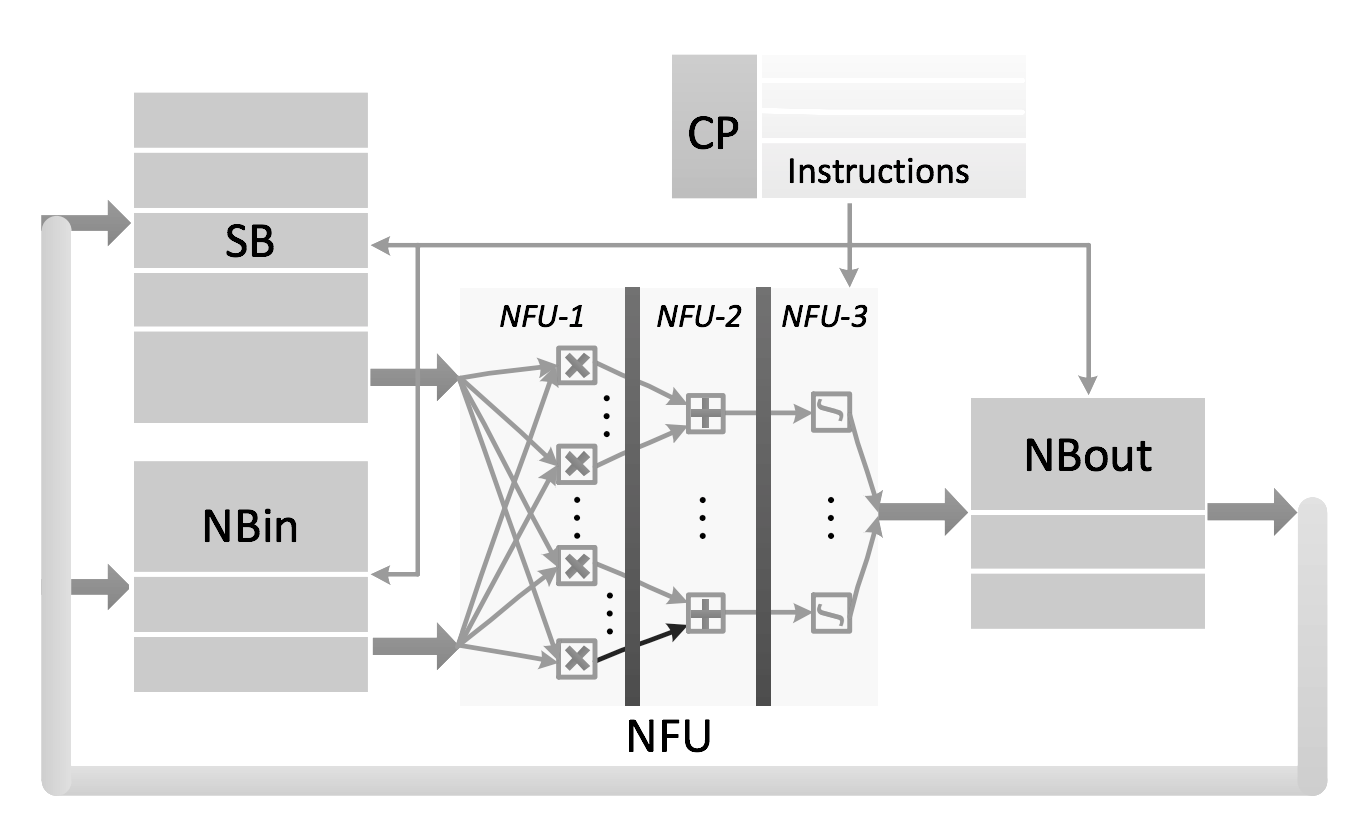
\includegraphics[scale=0.23]{./images/diannao.png}
	\centering
	\caption{Block diagram of the DianNao accelerator\cite{chen2014dadiannao}.}
	\label{fig:diannao_arch}
\end{figure}
To evaluate the performance of DianNao, Chen et al. structures two neural networks with similar architecture, but one with GPU (NVIDIA K20M) and the other one with DianNao acceleration. They also implemented the same network using CPU only without any acceleration. Figure \ref{fig:diannao_speedup} compares the speedup of GPU over both DianNao and CPU. It should be noted that the code for the GPU is developed using CUDA language and the CPU code is in C++ for different types of layers in the network.
\begin{figure}[h]
	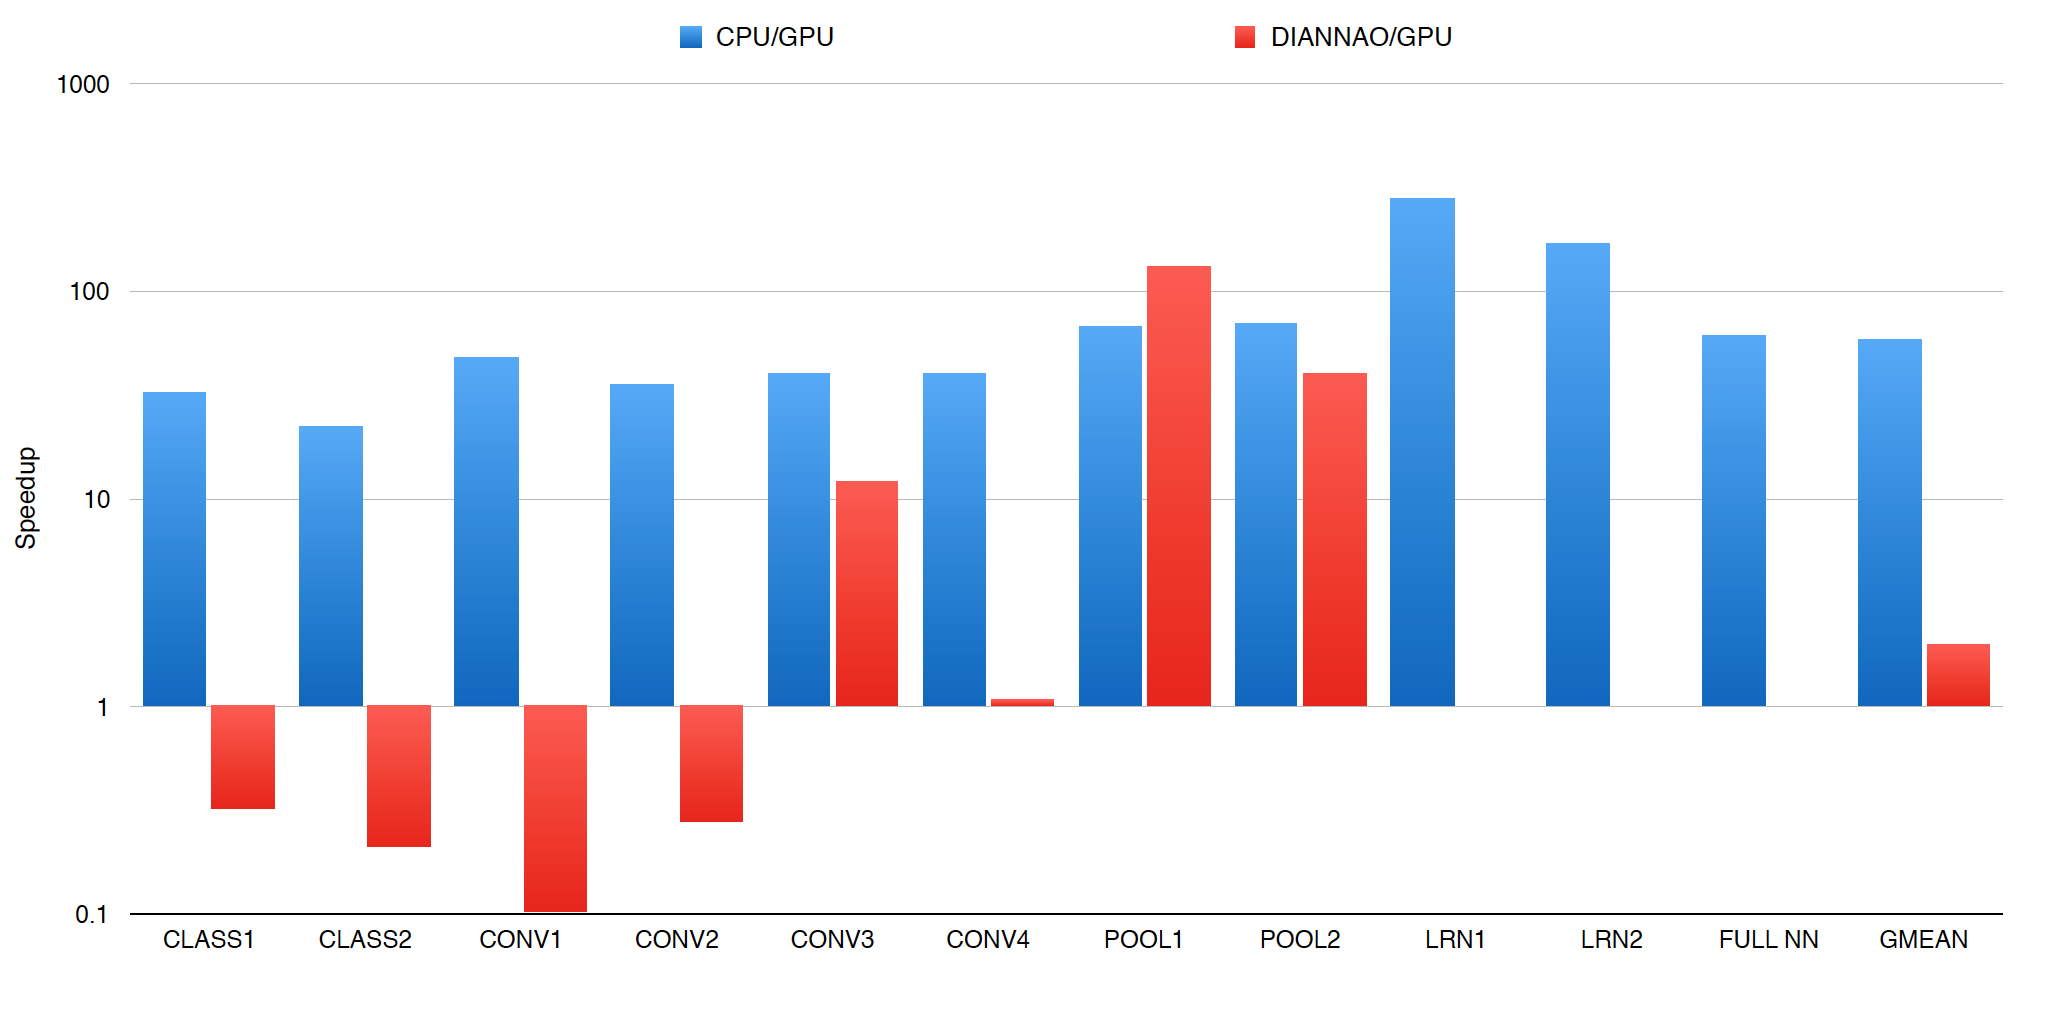
\includegraphics[width=\textwidth]{./images/diannao_results.png}
	\centering
	\caption{Speedup of CPU/GPU and CPU/DianNao for various layer types of network\cite{chen2014dadiannao}.}
	\label{fig:diannao_speedup}
\end{figure}

Figure \ref{fig:diannao_speedup} portrays that GPU has a speedup of around 50x to 100x for most layers. DianNao gives speedups up to 100 for some of the layers. However, in some other layers, mostly convolutional layers with private kernels and classification layers, which are common in both Deep Neural Networks (DNN) and Convolutional Neural Networks (CNN), GPUs may be preferred over DianNao. Authors believe that memory bandwidth is the major reason that DianNao performs worse than GPU in such layers. It should be noted that both convolutional and classification layers share the property that they have high number of synaptic connections in the range of millions. As DianNao takes up only about 53\% space of the a equivalent GPU, which is used for the sake of this comparison, it has shown the potential to compete with GPUs.
\subsection*{DaDianNao, the Machine Learning supercomputer}

DaDianNao is designed to serve as a Machine Learning supercomputer tailored for DNNs and CNNs. 
Dadiannao has a performance better or on a par with GPU options while taking up less area at lower costs. Besides, it can hold large models of even up to tens of GBs in size in a multi node structure.\\

As explained earlier, memory is thought to be the bottleneck of DianNao in convolutional layers with private kernel and classifier layers. The design of Dadiannao as a supercomputer aims to address these problems. First, in order to minimize data movement cost, synapses are placed near to the neurons consuming their data in a fully distributed architecture with no main memory unit. Secondly, nodes are designed so they tend to store instead of computation. Thirdly, since the number of synaptic connections is way more than the number of neurons,  instead of sending synaptic weights to neurons, neuron values are sent to synapses. This saves a lot in external communication bandwidth. Fourthly, intra-node, the storage units are broken into many storage units to increase the bandwidth.\\

The high level architecture of Dadiannao consist of many nodes arranged in a mesh configuration. Each node contains the storage units to store the synaptic and neuron values. In addition a, NFU unit is embedded similar to what introduced in DianNao \cite{chen2014diannao}.The NFU in Dadiannao is capable of carrying out more complex types of computation depending on the layers and mode of operation (training or inferencing). Figure \ref{fig:NFU_Diagram} shows the block diagram of a node for Dadiannao architecture. \\

\begin{figure}[h]
	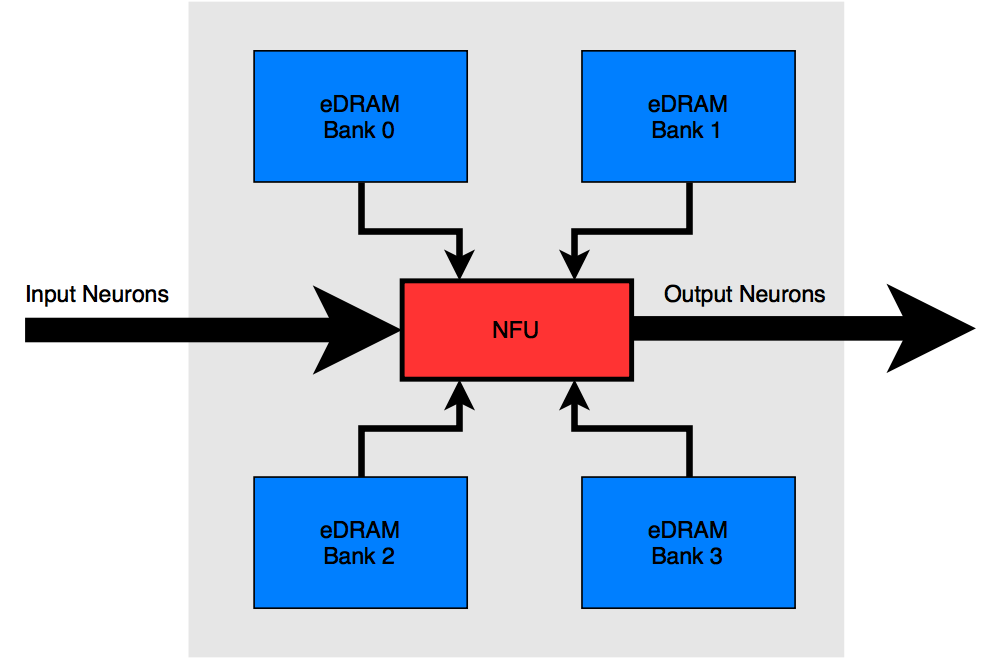
\includegraphics[scale=0.3]{./images/dadiannao_node.png}
	\centering
	\caption{Block diagram of a node within Dadiannao architecture \cite{chen2014dadiannao}.}
	\label{fig:NFU_Diagram}
\end{figure}
It should be noted that although SRAMs are generally preferred over other types of memory such as DRAM and eDRAM due to the higher speed, their size is limiting factor for them. A typical eDRAM can accommodate more than $2.5\times$ data compared to a SRAM. It should be noted that more storage density is required if parameters of big models are to be stored within chip to avoid external memory access. As a result, eDRAM is selected over SRAM in Dadiannao's proposed design. Refuting the memory bandwidth limitations for for computational units allows for scaling since more inputs and outputs to each neuron can be calculated simultaneously. However, eDRAMs suffer from some drawbacks compared to SRAMs namely, slower response, periodical refreshing requirement, and destructive read that may result in inaccurate values.\\

In order to exploit high bandwidth within nodes, a tile fashion layout is implemented as shown in figure \ref{fig:tiles}. In this design output neurons are assigned to various tile units. This enables NFUs to process data from multiple neurons in parallel.
\begin{figure}[h]
	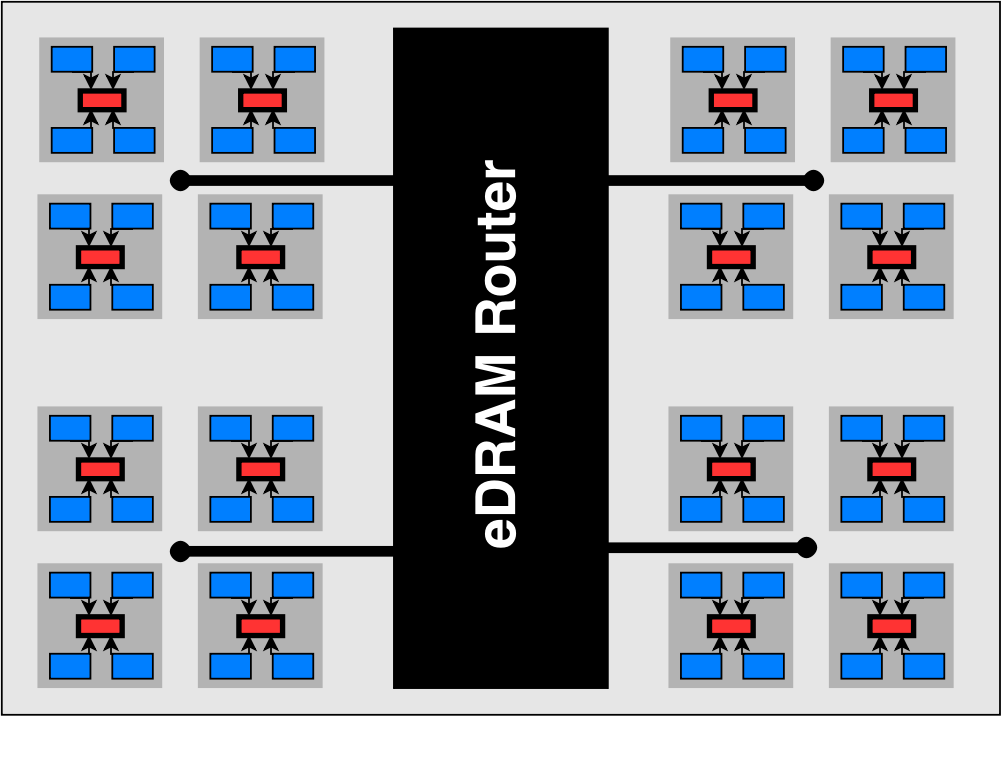
\includegraphics[scale=0.23]{./images/dadiannao_tile.png}
	\centering
	\caption{Tile implementation of a node \cite{chen2014dadiannao}.}
	\label{fig:tiles}
\end{figure}

Tiles in figure \ref{fig:tiles} are connected to eDRAM reservoirs in the middle, one for input neurons from tiles and one for output neurons. It should be noted that even though there are many tiles and NFUs in a node, the number of neurons in a typical Deep Learning architecture is much more to be a one to one relationship between NFUs and neurons. As a result, each NFU has the job of calculating many neuron outputs.

For most of the layer types, interconnect network of DaDianNao does not impose a bottleneck even despite the bulk number of neuron values, that has to be routed throughout the network. Hench, DaDianNao designer did not develop a custom-made network and adopted a 2D mesh topology with a HyperTransport 2.0 (HT2.0) IP block interconnection.

\subsection*{Experimental Results}
In this part we present the performance and energy consumption of Dadiannao. In figure \ref{fig:diannao_speedup}, performance of Dadiannao in the training mode is compared against its NVIDIA K20M GPU implementation counterpart.
\begin{figure}[h]
	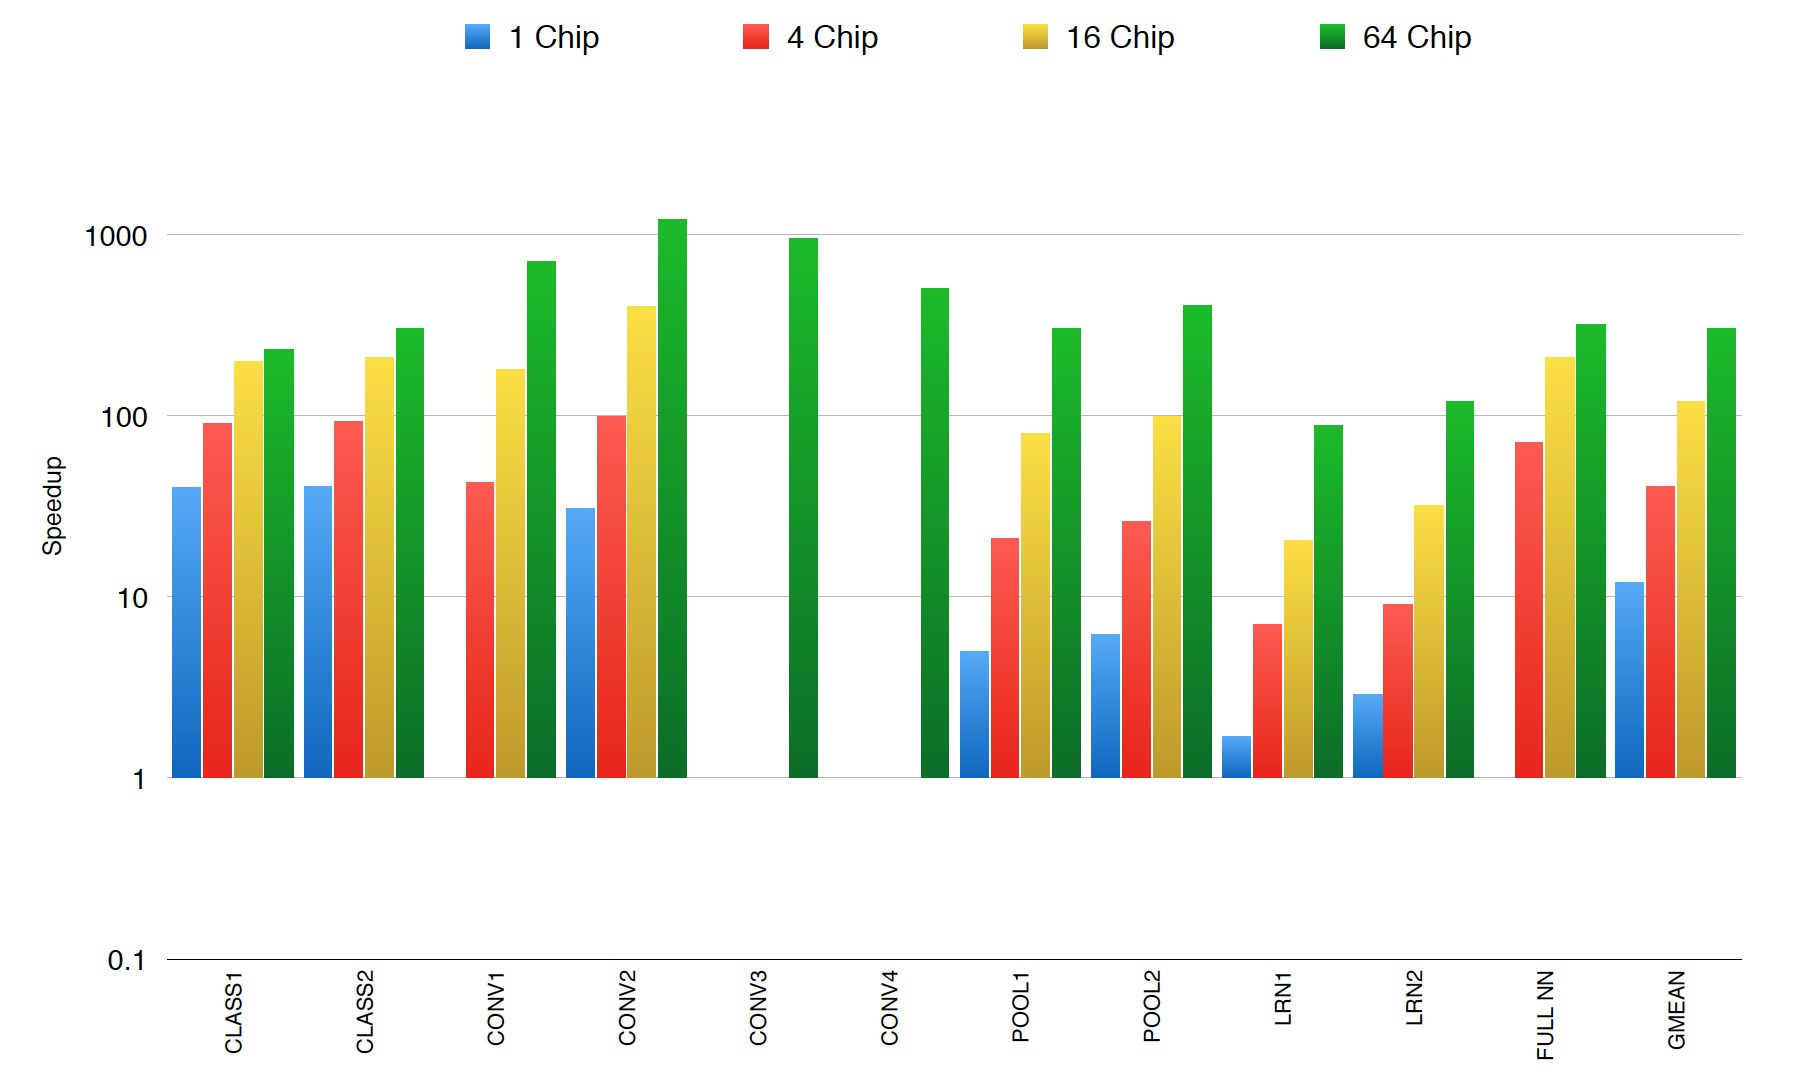
\includegraphics[width=\textwidth]{./images/dadiannao_chips.png}
	\centering
	\caption{Speedup of Dadiannao/GPU for various types of layers. CONV1 and fullNN layers require at least 4 nodes. CONV3 and CONV4 need at least 36 nodes to operate\cite{chen2014dadiannao}.}
	\label{fig:dadiannao_speedup}
\end{figure}

Figure \ref{fig:dadiannao_speedup} shows that Dadiannao could reach a speedup of more than 100 over the GPU system in almost all types of layers with 16 chips or more configuration. The speedup is even higher up to more than 1000 for the CONV1 and CONV2 layers when 64 chips are adopted. It should be noted that the size of CONV3 and CONV4 layers (which have private kernels) is relatively large in the range of GBs. As a result, the performance of these layers can only be measured with more than 36-node arrangement. The FULL NN layer, which is a fully connected layer also accounts for more than 50M synaptic connections and hence cannot be implemented on a system with only 1 node. Generally, average speedup of $21.38\times,$ $79.81\times,$ $216.72\times,$and $450.65\times$ is reported for Dadiannao over GPU for 1-node, 4-node, 16-node, and 64-node configurations, respectively. However, the speedup and scaling of various types of layers are wildly different due to the inherent characteristics of each type of layer.\\

In addition, the performance of DaAianNao against GPU baseline in evaluated from energy point of view. In the training mode the energy reduction rates against the GPU baseline are recorded as $172.39\times,$ $180.42\times,$ $142.59\times,$ and $66.94\times$ for the 1-node, 4-node, 16-node, and 64-node respectively. The energy reduction number reported in the inference mode is even higher. In the inference mode, the energy reduction for the 1-node, 4-node, 16-node, and 64-node configuration is $330.56\times,$ $323.74\times,$ $270.04\times$, and $150.31\times,$ respectively.


\section*{Conclusion and Outlook}
Machine Learning and Deep Learning have already become a part of our lives that we even do not notice them anymore. From search engines, voice recognition systems in our phones, and self-driving cars, all the way to commercial and financial analytics, they all benefit from machine learning and deep learning. With the help of fast CPUs and GPUs, training of models within Machine Learning and Deep Learning frame encountered a huge boost in the recent past. However, it seems that the future attempts to guarantee the scalability of such systems should also consider designing specialized software and hardware frameworks tailored to these applications such as project Adam and DaDianNao supercomputer.\\
\subsection{High Performance Graph Processing}
Graphs are abstract mathematical concepts that have numerous applications in science and engineering. Depending on the application and context they are being adopted in, they may have different types such a directed or undirected, cyclic or acyclic, finite or infinite, etc.\\
\begin{figure}[!ht]
	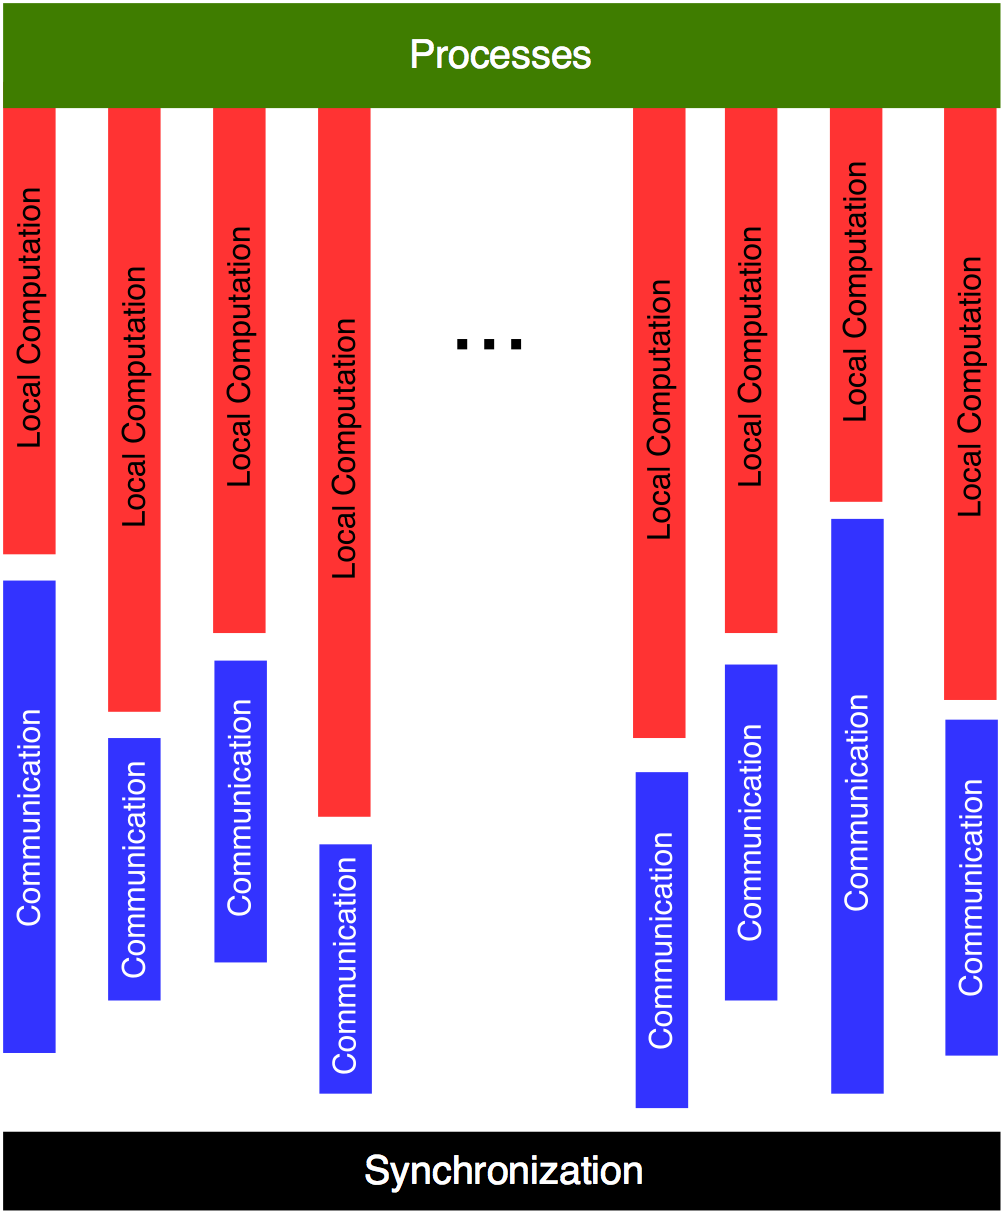
\includegraphics[scale=0.25]{./images/graph_multi.png}
	\centering
	\caption{Execution mechanism of BSP programming model.}
	\label{fig:BSP}
\end{figure}
With the explosion of data over the past decade, graphs have dictated themselves as tools with many interesting properties. Nowadays, graphs are an indispensable component of large data modeling systems. Graph databases are being more and more favored over relational databases with focus on relations as connections indicate foreign-keys in the traditional relational databases. Among many interesting inherent properties of graphs, their scalability is probably the most important distinguishing factor.\\

As Google's MapReduce originally designed to perform large volume data processing, heterogeneous commodity computer clusters can take advantage of MapReduce to run data analytics over hundreds of machines. On the other hand Hadoop implementation of MapReduce is not an optimal design for graph processing. As a result other graph processing technologies are suggested. Giraph \cite{avery2011giraph}, GraphLab \cite{low2014graphlab}, Apache Hama \cite{seo2010hama}, and GoldenOrb  are some of such technologies. In the remaining of this section we will briefly review Giraph and how it works.\\

Apache Giraph is inspired by Google Pregel \cite{malewicz2010pregel} at yahoo and donated to Apache Software Foundation (ASF) later. Giraph jobs can easily be run on Hadoop within a cluster. Depending on the version of Hadoop in use it can either employ mappers or execution containers from Yarn. Giraph adopts a Vertex-centric API approach to perform the processes, which is inspired by the Bulk Synchronous Parallel (BSP) programming model. It means that vertices send and receive value from other vertices. During a series of iterations called \textit{supersteps}, at each iteration a vetix is executed with a user-defined function. Vertices receive messages from other vertices in the past executions. Respectively they send messages to other vertices to be executed in the next iteration. Figure \ref{fig:BSP} depicts the execution of computations using BSP.

Each vertex has the option of becoming active or inactive during each iteration. If a vertex does not receive a message it can vote to halt and become inactive. Similarly, an inactive can become active upon arrival of a message. The overall execution continues until no vertex has a message to send. Figure \ref{fig:max_super} illustrates an example of finding the maximum value in a graph.

\begin{figure}[!ht]
	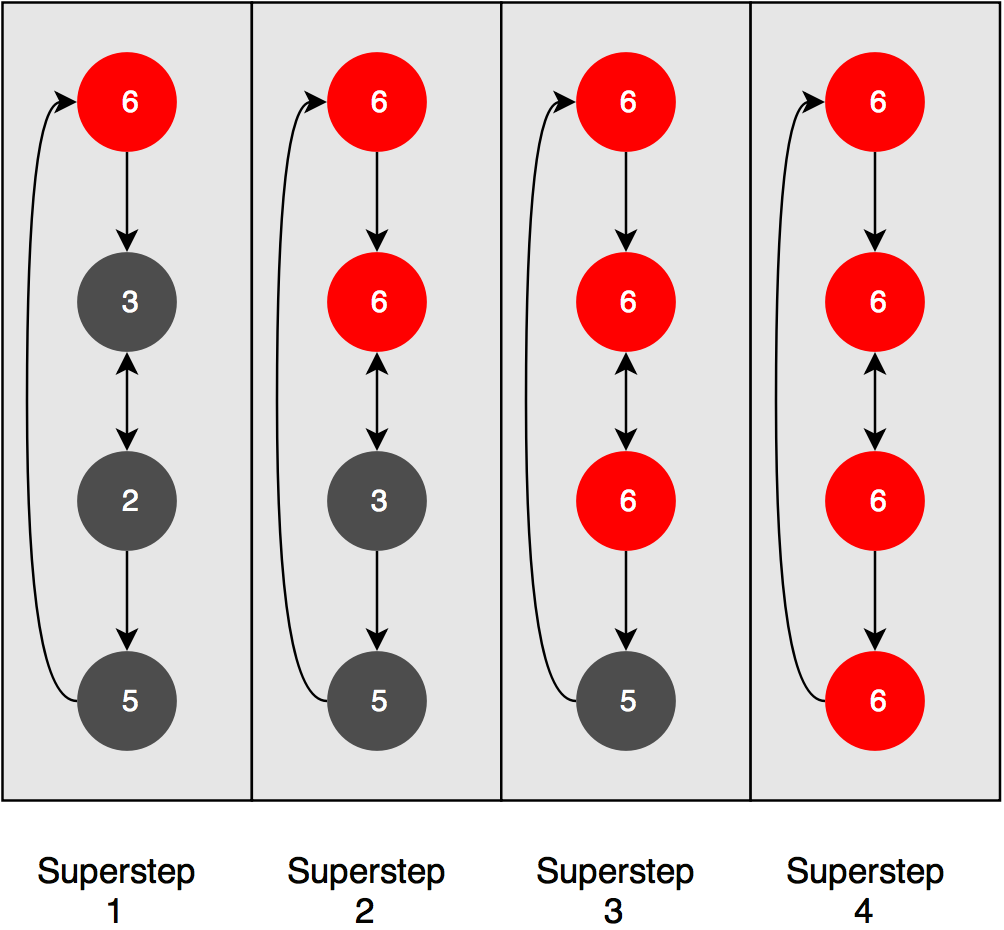
\includegraphics[scale=0.23]{./images/graph_superstep.png}
	\centering
	\caption{Example of computing maximum vertex value. At each superstep values for each vertex are sent to the neighbor. If the received value is higher than the current value, current value is updated. Otherwise, current value is hold \cite{sakr2013processing}.}
	\label{fig:max_super}
\end{figure}

%%%%%%% KRUNAL ADDED
\subsection{Parallel Databases and I/O}
Although the idea of parallel database system was refuted by a  \cite{dewitt1983database} DeWitt \textit{et al.} in 1983, prophesying demise of database machine, that did not stop widespread adoption of parallel database. Companies like Teradata, Tandem and many other startups pioneered a path for successful parallel database systems. The evolution to parallel databases fated due to wide adoption of relational model which favors the idea of parallel dataflow graph, leading to pipelined parallelism and partitioned parallelism. Based on the market trends, ten years later in \cite{dewitt1992parallel} DeWitt \textit{et al.} explains how parallel database system will be the future of high performance database systems. With the advances in high speed interconnect network, the client-server architecture gave much higher performance over price than its mainframe equivalent.\\

A parallel database system can be classified based on the terms of how data is shared amongst multiprocessor system i.e. shared-memory, shared-disk or shared-nothing. By the early 90's, it was clear that shared-nothing architecture along with conventional processor, memories and disk would be the future of scalable parallel and distributed system. Linear speedup and linear scaleup are two characteristics of an ideal parallel database system. But usually a sub optimal speedup and scaleup is observed due to these three issues: startup, interference and skew. SQL language was introduced by Codd, in his historic paper, to support data independence and boost programmer's productivity by separating execution logic from query itself. However, it came along with added benefits of parallelism, making it possible to represent each relational operator on a data flow graph and dividing data into a parallel data streams for partitioning. There are several partitioning strategies like round-robin, hash, range partitioning etc. \\

Although, there is a heated argument about the performance benefits of using a Map Reduce system against the parallel DBMS system, former has been widely adopted because it offers better performance with complex queries on unstructured data. High performance computing systems have high speed network, parallel file systems and diskless nodes while Big data analytics research has evolved from an increasing demand for extracting knowledge from large data set on a big or small cluster with low speed network and each node its own disk with local file system. For example, Lustre file system is widely used in HPC environment whereas Hadoop's HDFS is one of the popular choice for big data analytic applications. The main focus of HPC systems is to optimize and exploit the resources, with a parallel file system. During the past decade, several attempts are made to bridge the gap between HPC and Big data analytics research, giving rise to new terms like High Performance Data Analysis. In the next section, we discuss about some of these research that has been propelled towards amalgamation of these two giants.\\

\subsection*{SCOPE}

Structure Computation Optimization for Parallel Execution (Scope) is a distributed computing system, that incorporates best characteristics of traditional parallel database system and map reduce execution engine, like scalability and robust implementation. In \cite{zhou2012scope}, the author describe about SCOPE's architecture and optimization techniques to achieve better performance. 
It uses SQL like query language to embrace relational query optimization techniques and separate application logic from underline implementation on a distributed system. It supports both structured and unstructured stream. All the execution plan are generated by a cost-based optimization system which is scheduled by a job scheduler, similar to MapReduce system. SCOPE runs on top of COSMOS (a distributed data platform), and used in many on-line service from Microsoft like Bing. \\

\begin{figure}[!ht]
	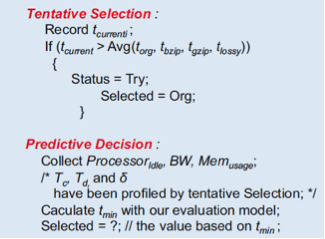
\includegraphics[scale=0.5]{./images/krunal8.png}
	\centering
	\caption{Architecture of COSMOS with three main components\cite{zhou2012scope}.}
	\label{fig:krunal8}
\end{figure}

\subsubsection*{COSMOS: }
Figure \ref{fig:krunal8} shows the architecture for COSMOS platform which can be divided into three main components: Storage system, Computing system and Frontend services. COSMOS storage system is a distributed append-only file system which provides fault tolerance by data replication and reliability for storing petabytes of data. Writes are always append-only and serialization is used for concurrent writes. The storage system consist of a physical partitions called extends, which is the unit of space allocation and replication, typically a size of few 100 MB. Application extends are often compressed and decompressed at client side, contains application-defined records and define a block boundary. Local or remote read and write are enabled through high-bandwidth network. Directed acyclic graph (DAG) are used for modeling a query plan. Job submission/management, job queue monitoring, job status tracking, error reporting and transferring data in and out of COSMOS are done through an interface provided by front-end services. \\

\subsubsection*{Data Representation and Query Language: }
Unstructured stream are defined as a logical sequence of bytes that requires an extractor for users to interpret it. An extractor defines the schema and iterator interface for transforming the data. It also provides an outputters that writes output in an unstructured streams. Structured stream are handled by build-in function that allow an unvarying access time by storing data with into different schema which is self-contained, that is, with rich metadata information such as schemes, structural properties and access method. Usually data is horizontally partitioned with different schemes like hash and range partitioning. Each structural stream consist of several physical extents which allows effective replication and fault tolerance. Data is stored based on store affinity and assigned affinity id, each affinity group having same id. Storage priority is given first at same machine level and if the storage is full then at same rank until its saturated and then at next close rank.  Another optimization to improve performance is stream references, in this technique the output stream is referenced with another corresponding partition based on affinity id according to storage priority. It also supports techniques like Indexing for random access, column group for vertical partitioning, etc.  \\

SCOPE query language resembles SQL and has many SQL-like extensions that enable users to separate application logic from underline implementation on a distributed system. For unstructured stream, it provides personalized commands for EXTRACT and OUTPUT, for reading from source and writing data to a sink. Structure stream removes the constraints of specifying columns because it is already contained in the stream metadata during compilation. Reference clause can be used to specify affinity of output to another stream. REDUCE command can be replaced by adding an optional PRESORT and PRODUCE clause. Figure \ref{fig:compilation_of_a_scope} shows the all steps of transformation for a SCOPE script before executing in the cluster. 

\begin{figure}[!htb]
	\includegraphics[scale=0.5]{./images/krunal2}
	\centering
	\caption{Compilation of a SCOPE script.}
	\label{fig:compilation_of_a_scope}
\end{figure}

\subsubsection{Code Generation and Runtime Engine: }
SCOPE runtime engine supports all the relational operators along with build in and optimized UDOs(User Defined Opcodes) like DefaultTextExtractor and DefaultTextOutputter. Simple functions like open, next and close are performed by operator which inherently supports pipelining of these operators.  The runtime engine, after optimization, generates a physical execution tree by doing these tasks:
\begin{enumerate}
	\item The whole plan is analyzed to produce corresponding codes for operator based on the internal operator template.
	\item  Output tree is partitioned at exchanges and spool operations to generate a super vertex that contains a series of physical exchanges.
	\item Break large super vertex into smaller ones to avoid skew delay due to longer execution time.
	\item An assembly is made by compiling all the generated code into it and the entry functions for each super vertex is written into super vertex definition.
	\item Each super-vertex is schedule to execute on a single machine.
	\item Like traditional db system, a queue of additional super vertices are maintained through admission control technique when all resources are allocated.
\end{enumerate}

Compilation script output consist of three components:
\begin{enumerate}
	\item Algebra file: Enumeration of all super-vertex and the data flow relationship between them.
	\item Super vertex definition file: Specification and entry point in the generated code for all super vertex.
	\item Assembly: Contains the generated code.
\end{enumerate}

\subsubsection{Execution Model: }
Similar to MapReduce, SCOPE implements a pull execution model. Super vertex, that reads data either locally or remotely, are executed in a pipelined fashion with an end result written to a local disk and waiting for the next vertex to pull data. This approach contrast with the execution model of parallel database which transfer intermediate data directly without any disk access. However, pull execution model has an advantage that both parties involved in data exchange need not run simultaneously and the data can be recovered from disk on failure. Since shuffling of data is the most expensive part considering the network overhead, SCOPE runtime provided many partitioning and merge operators.  It supports hash, range and index-based partitioning, with number of partitions either predetermined or determined based on intermediate data size during runtime.\\

\subsubsection{Job Scheduling: }
SCOPE's job manager is an adaption from Dryad, which takes care of job graph and resource scheduling on clusters. DAG of super vertices is scheduled to execute separately on different machines. Vertices are classified into different stages by Job manager and all the vertices in a single stage perform same task.  Data storage and computation can be performed by all the machine.
\begin{figure}[!htb]
	\includegraphics[scale=0.4]{./images/krunal3_new}
	\centering
	\caption{SCOPE job scheduling }
	\label{fig:scope_job_sched}
\end{figure}
Local system resources are maintained by processing node services and it also schedules execution of local vertices along with monitoring state of a job. Based on available resources and priorities it generates process on behalf of job managers and maintains a local queues of vertex execution request from different job manager. It stores the assembly of vertex in a cache so it can be used if the vertex is executed again. An initial DAF is formed, when the job begins, to oversee relationship among different vertex. According to execution results and variation in system environment, the job graph can dynamically adapt itself. Resource availability and vertex priority defines the actual vertex scheduling order and it's the task of job manager to notify any vertex execution failure.\\

\subsection*{Adaptive Hybrid OLAP Architecture}

Since last decade, co-processor technology has evolved rapid due to huge demand of high resolution and graphic intensive games. These co-processors are very good at processing computationally intensive tasks and since data analytics usually requires a single operation on a multiple datasets (SIMD), it's turns out to be perfect candidate. In the most of the research, the CPU ( device) acts as a supervisor and GPU (host) carries out all the task which leads to inefficient use of device resources. \\

An adaptive hybrid OLAP (On-line Analytical Processing) architecture is proposed in \cite{riha2013adaptive} that uses prediction model to efficiently distribute and process data on CPU and GPU based on their memory subsystem and memory access pattern. OLAP has a fundamental structure of a data cube which consist of multi-dimensional data that enables user to explore relation amongst different aspects of data. Data is partitioned into two types of OLAP cubes for processing on CPU and GPU:\\
\begin{enumerate}
	\item Multidimensional OLAP (MOLAP): These cubes contains preprocessed data that is sparse and huge in size. It is coherent to CPU's memory system.
	\item Relational OLAP (ROLAP): It contains data that is manipulated to appear like traditional OLAP with slicing and dicing functionality, which makes it suitable to be processed on GPU architecture.
\end{enumerate}

 A single CPU's main memory cannot accommodate all the MOLAP cuboids, due to their large size, so it spans multiple CPUs (each having a separate memory controller) which leads to a NUMA (non-uniform memory access) architecture, show in figure \ref{fig:nume_something}. This results into a memory bandwidth constraint of processing OLAP on CPU, because of the distribution of data as shown in figure 2. So usually all the queries for which cuboids are not pre-calculated gets handled by GPU.
 
 \begin{figure}[!htb]
 	\includegraphics[scale=0.5]{./images/krunal4}
 	\centering
 	\caption{The NUMA (Non-Uniform Memory Access) effect in two CPU with private memory and memory controller. The system has a shared memory address space but memory access has non uniform latency. Each processor has quicker access to its own physical memory and some delay while accessing other CPU's physical memory }
 	\label{fig:nume_something}
 \end{figure}

\begin{figure}[!htb]
	\includegraphics[scale=0.4]{./images/krunal5_new}
	\centering
	\caption{Sub-Cube is partitioned amongst two physical memory. Scenario 1 shows the most ideal case where partitions are equally distributed. Scenario 2 show a suboptimal case where either of the CPU have only 25\% of the data. And 3rd scenario shows worst case when a whole sub-cube is inside only single CPU's memory. }
	\label{fig:Cuboid_divide}
\end{figure}

Star scheme is used for processing ROLAP cube queries and the fact tables are stored inside GPU's main memory. These fact table contains two columns:
\begin{enumerate}
	\item Dimension columns for indexing
	\item Data columns that stores the OLAP cube. 
\end{enumerate}

The device handles MOLAP cuboid queries along with other query processing tasks like query translation and dimensional table search. After the dimension tables are processed on the CPU, corresponding fact table entries are handled by GPU using values in dimension column.\\

A scheduler predicts whether to use CPU or GPU based on current utilization statistics, estimated query processing time on both the architectures and availability of data. Figure \ref{fig:krunal6}, shows the block diagram of system partition and scheduler distributing six different partitions on GPU. The CPU query processing time is estimated from the size and location of the sub-cube as well as memory bandwidth for multi-dimensional data representation. Data compression plays a vital part considering the bottleneck of data bandwidth. Strings are converted into integers by creating a dictionaries of unique string for each column and the dimension table contains the indices of these string from respective dictionaries.
\begin{figure}[!htb]
	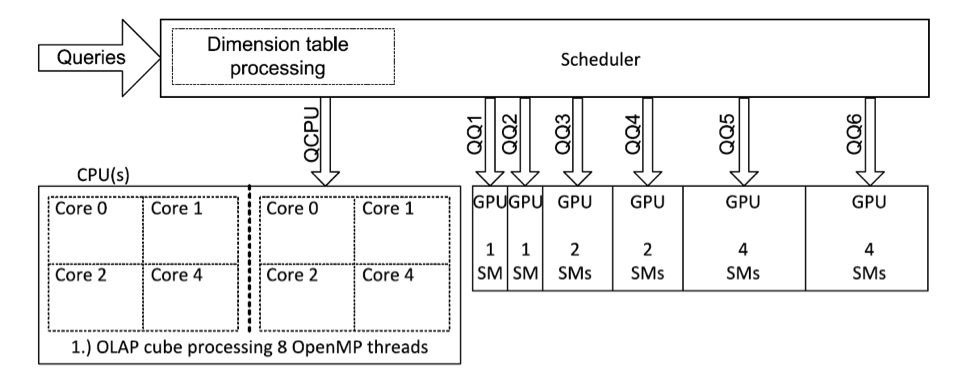
\includegraphics[scale=0.3]{./images/krunal6}
	\centering
	\caption{Block diagram of system partition. The scheduler assigns MOLAP cube processing task to CPU and all the queries on fact table are directed to GPU partitions. Each GPU partition contains different number of streaming processor(SM)   \cite{riha2013adaptive}}
	\label{fig:krunal6}
\end{figure}

\subsection*{Improving IO performance with Adaptive Compression}
With the NUMA architecture, discussed in previous section, a large amount of I/O operations is transferred from one node's memory to either another node's memory or directly to storage. In some compute intensive prediction applications, like simulation analysis, there can also be some staging nodes and I/O nodes to perform analysis and data storage respectively. Figure \ref{fig:krunal7}  shows a block diagram of different stages in simulation analysis. \\
\begin{figure}[!htb]
	\includegraphics[scale=0.4]{./images/krunal7_new}
	\centering
	\caption{Nodes are arranged into three level in simulation analysis. Compute nodes can carry out simulation and some nodes act as a helper nodes performing intermediate analytics. Staging nodes only performs analytics and their output is passed on to I/O nodes, responsible for storage. Label 1, 2 and 3 point out the  tentative adaptive compression location in simulation analysis.}
	\label{fig:krunal7}
	\end{figure}
	
All these communication are slow compared to the computational process time and usually becomes an overhead. It can be addressed by increasing in-situ analysis and decreasing the amount of data transfer. Big data application usually results into high IO and one way to limit this overhead is through compression. The selection of best compression algorithm can be done based on different parameters like system resources, data type and type of compression (lossy or lossless) feasible. Compression can be applied at different stages of data analysis process as shown in figure \ref{fig:krunal7}. However, the compression process is resource and time consuming while at the same time system resources can vary and so can the type of transfer data. It can be possible that time to compress the data and transfer time added up to be more than the actual time to transfer uncompressed data, making compression an overhead itself.\\

 \cite{zou2014improving} discusses about an adaptive data compression method that uses a hybrid technique to predict and apply efficient compression algorithm at each data transfer round. It combines two different algorithms, tentative selecting compression algorithm and predictive deciding compression algorithm, to device an optimal compression technique. The tentative selecting compression technique profiles the compression speed and ratio of the compression at the beginning of each round by sending some data blocks that can contain compressed or actual data. Based on the tentative latency an optimal algorithm is chosen. This algorithm, show below, is simple to implement but does not take into account resource status.\\

	\begin{algorithm}
		\caption{Tentative Selection}\label{tentative}
		During the beginning of each round
		\begin{algorithmic}[1]
				
			\item Record current time latency
			
			\item Find tentative time latency for all the candidate algorithm (bzip, gzip,lossy, etc)
			\item If current latency is greater than other technique, select the best compression algorithm based on the tentative latency
			
		\end{algorithmic}
	\end{algorithm}
	
	\begin{algorithm}
		\caption{Predictive Decision}\label{predictive}
		\begin{algorithmic}[1]
			
			\item Measure all the required metrics (Processor cycles, compression/decompression throughput, Compression Ratio, Available data transfer bandwidth and memory impact factor)
			
			\item  Use evaluation model to calculate Minimum time (Tmin)
			\item  Based on the value of Tmin select a compression algorithm
			
		\end{algorithmic}
	\end{algorithm}



Predictive deciding algorithm selects the best algorithm based on the change in resource status during each round. The algorithm, shown above, relies on a quantitative pre-build algorithm evaluation model, which includes metrics like available processor cycles, available transfer bandwidth and memory impact factors. It produces some overhead while monitoring real-time resource status but does not predict the best compression technique when the data format changes. Figure \ref{fig:krunal9} depicts three rounds, separated by black vertical lines, of data compression and transfer instructed by tentative and predictive implementation called T$\_$Selection and P$\_$Decision respectively. T$\_$Selection can accurately predict change in compression technique but it needs to check all the techniques at the beginning of the each round whereas P$\_$Decision does not have such extra overhead during each round but its prediction is not always accurate. \\

\begin{figure}[!htb]
	\includegraphics[scale=0.5]{./images/krunal9_new}
	\centering
	\caption{Data compression and transfer analysis of two implementation and adaptive hybrid implementation.}
	\label{fig:krunal9}
\end{figure}

A hybrid technique amalgamates best of both i.e. performance profiling and resource monitoring together into one comprehensive method. Resource variation leads to change in algorithm by a predictive decision in real-time and tentative selections are carried out simultaneous with data compression selection after every threshold time interval (T\_round). Figure \ref{fig:krunal9} also shows the adaptive data compression and transfer analysis used in this hybrid technique along side previous unoptimized implementations.\\

\newpage
\subsection{HPC implementation of MapReduce}
As we know now, MapReduce as a programming model is based on functional programming paradigm. MapReduce programming model is a good fit for applications where large amounts of data on many nodes require to be processed. MapReduce programming model facilitates parallel processing of data since execution of mapper and reducer function on each node, which comprise key-value pairs is embarrassingly parallel. However, during the sort/shuffle stage when output of mapper functions has to be routed toward the inputs of articular reducers, some communication overhead is introduced.\\

Hadoop implementation of MapReduce is currently the most widely used tool in data centers. As map and reduce processes are distributed across a cluster of machines, data require high performance, reliable, and fast processing and communication among machines across the cluster. HPC technologies can assist current Big Data architectures through the following approaches,
\begin{itemize}
	\item \textbf{Accelerators:} Employing hardware accelerators like GPUs, FPGAs, and CPUs.\\
	\item \textbf{Hardware modifications:} Adoption of efficient high throughput HPC networks such as InfiniBand through modified memory space structures like Remote Direct Memory Access (RDMA).\\
	\item \textbf{Software modifications:} Taking advantage of alternative HPC programming models such as Partitioned Global Address Space (PGAS).\\
\end{itemize}
In the following part we will give two examples of MapReduce implementation from literature. The first example is a RDMA-enabled implementation of MapReduce and the second example utilizes X10 as a PGAS programming language to implement MapReduce.\\


InfiniBand as a high performance interconnect has been quite known to HPC community for more than a decade now. In \cite{wasi2013high} \textit{Rahman et al} showed that a native InfiniBand using Remote Direct Memory Access RDMA for a 100GB TeraSort on eight nodes achieved a performance improvement of 32\% over IP-over InfiniBand (IPoIB) and 21\% over Hadoop. Figure \ref{fig:RDMA_hadoop} shows the architecture of the proposed structure.
\begin{figure}[!htb]
	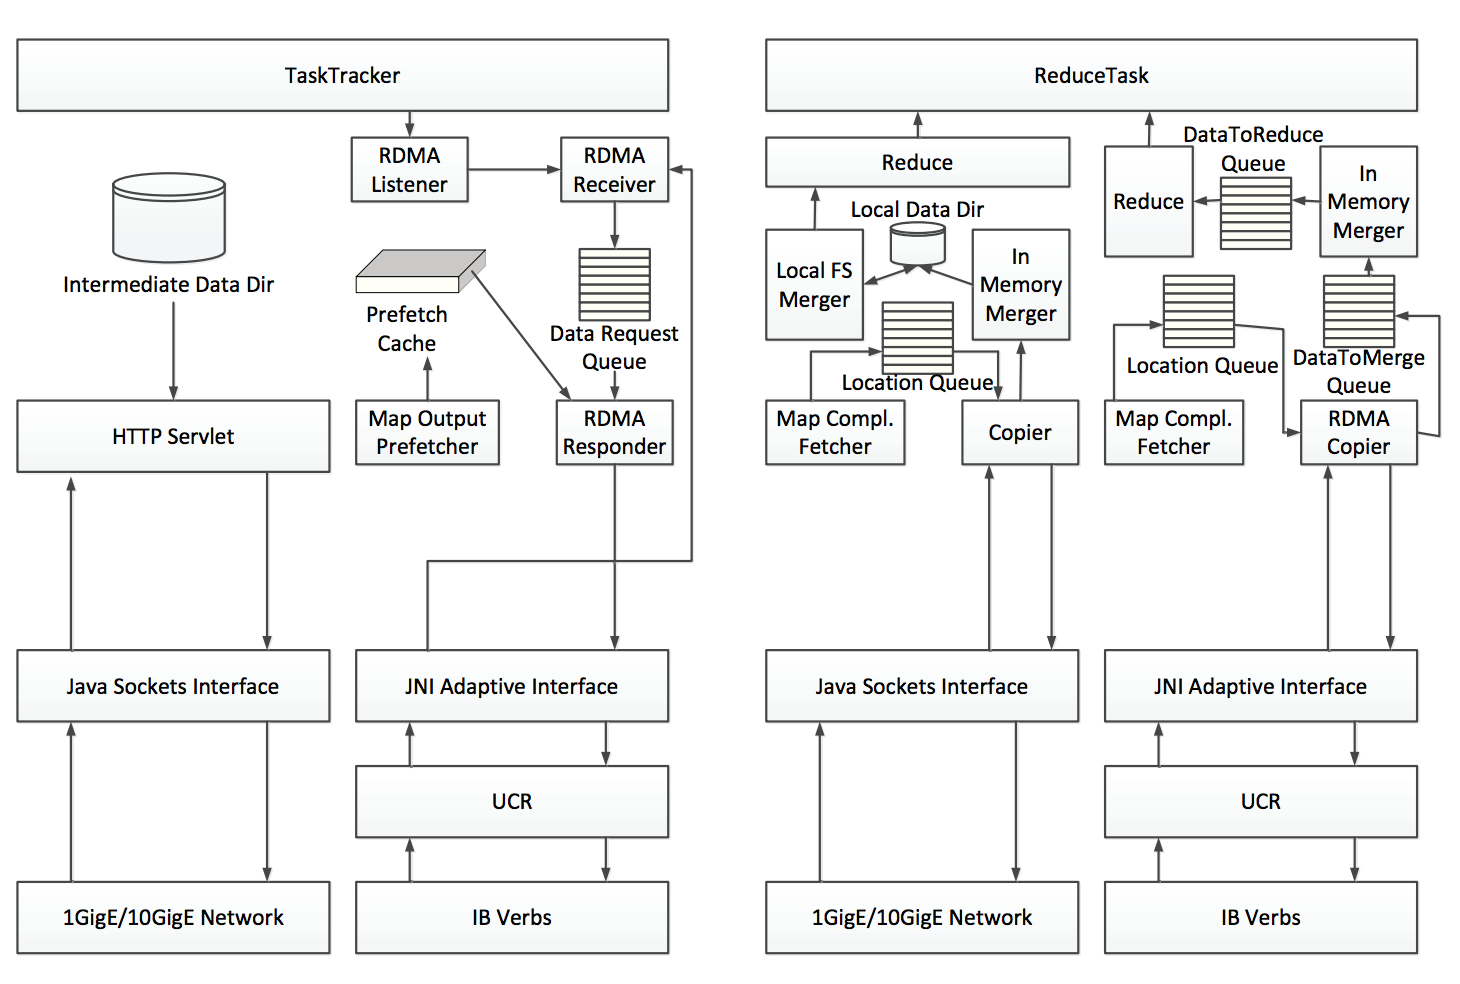
\includegraphics[width=\textwidth]{./images/RDMA_Hadoop}
	\centering
	\caption{RDMA based architecture of MapReduce proposed by \cite{wasi2013high}.}
	\label{fig:RDMA_hadoop}
\end{figure}
The proposed architecture in Figure \ref{fig:RDMA_hadoop} adopts a modified Shuffle and Merge design. For the RDMA based Shuffle many components are added. For instance, RDMAListener, which is initiated by on the TaskTracker side listens to connection requests that arrive from ReduceTask side and assigns a receiving request from RDMAReceiver if needed. The RDMAReceiver then forwards the request to DataRequestQueue. Requests staked at DataRequestQueue are sent to RDMAResponder for processing. On the ReduceTask side the RDMACopier submits requests to TaskTracker and as the data arrives, DataToMergeQueue will take it for merge processes. Modified merge design in the proposed architecture benefits significantly from the high performance networking. As the communication time is reduced, key-value pairs in the map outputs can be sent over many steps. Thus, reducers may start processes on a stream of key-value pairs as they arrive.\\

The proposed design is improved the execution time by 21\% over Hadoop with 100GB TeraSort. The reported improvement for a 40GB regular Sort is 32\%, which is more than that of TeraSort. The design also took other optimizations such a efficient pre-fetching and caching. The authors are planning to enhance other features such as recovery time upon failure and evaluating their design on bigger clusters for more diverse number of applications.\\

As we mentioned earlier, another approach for taking advantage of HPC capabilities is the software approach. PGAS programming model is one of the best fits for parallel programming. PGAS programming model allows for a global shared memory architecture while affinity of a memory location to processor/thread is transparent. The latter enables processes to take advantage of locality of data to deliver higher performances.\\

In \cite{teijeiro2011design} Teijeiro \textit{et al.} implemented a parallel MapReduce using Unified Parallel C (UPC) \cite{el2006upc} programming language. UPC enables uniform parallel programming paradigm along with powerful C language features. The UPC implementation of MapReduce defines two sets of functions namely, generic management functions and user-defined functions. Generic management functions start and control basic setup and data distribution task withing both Map and Reduce stages. In contrast, user-defined functions enable to processing on elements from output of Map stage, intermediate stage, to the input of the Reduce stage. Generic Map function enables threads to be aware of all input elements. However, each thread is only given a fraction of those input elements. After each thread completes its processing task in the Map stage, the resulted intermediate values hold in a private memory for future processing in the following steps.\\

At the Reduce stage, each thread should be told whether or not it is in possession of all the values required for the reduction or not. If all the threads have all the necessary values. no communication happens. Otherwise, each thread is provided with a thread number, which it has to communicate with in order to retrieve values it need for reduction.\\

The performance of the UPC implementation of MapReduce is compared to that of an MPI based design for two application namely, Word Count and Histogram. The Word Count experiment essentially counts the appearance of each distinct word in a text input. The Histogram experiment comprises calculating the histogram for pixel values in a bitmap image. The results from Word Count experiment showed that the execution time for UPC implementation is only slightly better than MPI implementation for fewer number of threads. In addition as the number of threads increase beyond a point, MPI execution time become less than UPC. In contrast, for the Histogram experiment, the UPC execution time is improved up to more than two orders of magnitude compared to the MPI implementation. In conclusion, authors believe that the enhanced performance of UPC im	plementation is due to  generic and simple UPC frameworks. In addition the better programmability of UPC with the high performance can be the motivation behind using PGAS implementation of MapReduce. 



\section{Future Direction}
%In the last two sections of this chapter we described what big data is and reviewed some of the state of the art projects in the big data domain. In this section we will try to discuss major challenges ahead and directions to get past them. In order to keep consistency, we address challenges and direction we regards to the big data characteristics we introduced earlier in this chapter as 5Vs. 
%
%\subsection{Variety:} Most of the available data today is stored in a variety of types and formats as video, picture, audio, clicks, numbers, likes, tweets, etc. Even when we narrow down our search to a very specific group of data
%%%%%%%%%%%%%%%%%%%%%%%%%%%%%%%%%%%%%%%%%%%%%%%%%%%%%%%%%%%%%%%%%%%%%%%%%%%%%%%
\newpage
\bibliographystyle{splncs03}
\bibliography{paper_2.bib}

All links were last followed on October 5, 2014.
%%%%%%%%%%%%%%%%%%%%%%%%%%%%%%%%%%%%%%%%%%%%%%%%%%%%%%%%%%%%%%%%%%%%%%%%%%%%%%%
\nocite{*}
\end{document}
